\documentclass[
        oneside,      %%coloque  % no in\'icio desta linha para imprimir frente e verso 
        english,			
%	french,				
%	spanish, 
        brazil			 
        ]{abntbibufjf}


\usepackage[T1]{fontenc}		
\usepackage[utf8]{inputenc}		%% Para converter automaticamente acentos como digitados normalmente no teclado. Mude utf8 para latin1 se precisar. 

\usepackage{lmodern} %no caso do modelo Latex, pode-se usar a fam\'ilia de fontes lmodern como aqui indicado, no lugar de Arial e Times New Roman.


\usepackage{lastpage}			
\usepackage{indentfirst}		
\usepackage{color}			
\usepackage{graphicx}			
\usepackage{microtype} 
\usepackage{hyperref}
\usepackage{xurl}
\usepackage{amssymb}
% --- Matemática (necessário para \text, \operatorname, \lVert, etc.)
\usepackage{amsmath}
\usepackage{amssymb}
\usepackage{amsfonts}
\usepackage{float}

\usepackage{listings}
\usepackage{xcolor}


% Configuração do estilo para Python
\lstset{
  language=Python,
  basicstyle=\ttfamily\small,
  keywordstyle=\color{blue},
  stringstyle=\color{red!70!black},
  commentstyle=\color{green!50!black}\itshape,
  numberstyle=\tiny\color{gray},
  numbers=left,
  stepnumber=1,
  numbersep=8pt,
  backgroundcolor=\color{gray!10},
  frame=single,
  tabsize=4,
  showstringspaces=false,
  breaklines=true,
  captionpos=b
}

%% -----------------------------------------------------------------------------

%% Obs.: Alguns acentos foram omitidos.

\titulo{Identificação do Ideal Customer Profile em Negócios B2B} 
\subtitulo{Modelo Computacional Aplicado ao Setor de Benefícios Corporativos}  %% Colocar % no in\'icio desta linha se nao tiver subt\'itulo 
\autor{Félix Oliveira Miranda} %%Colocar, dentro de chaves {}, o nome completo do autor
\autorVirg{Miranda, Félix Oliveira} %%Colocar o sobrenome do autor, separado por v\'rgula, antes do restante do nome do autor. Ex.: Santos, Maria dos
\local{Juiz de Fora} %%Governador Valadares % N\~ao usar MG.
\data{2025} %%Colocar o ano da entrega. Por exemplo, 2019. N\~ao usar m\^es.
\orientador[Orientadora:]{Priscila Vanessa Zabala Capriles Golliat} %%Se precisar, troque [Orientador:] por [Orientadora:]
%\coorientador[Coorientador:]{Nome e sobrenome} %% Colocar ``%'' no in\'icio desta linha se n\~ao tiver coorientador. Se precisar, troque por [Cooorientadora:]. 
\orientadorTitulo{Profa. Dra.} %%Colocar, dentro de chaves {}, a titula\c{c}\~ao do(a) orientador(a). Por exemplo, Prof. Dr.
%\coorientadorTitulo{Titula\c{c}\~ao} %%Colocar, dentro de chaves {}, a titula\c{c}\~ao do(a) cooorientador(a). 
\instituicao{Universidade Federal de Juiz de Fora}
\faculdade{Faculdade de Engenharia} %%Colocar, dentro de chaves {}, o nome da faculdade ou do instituto.
\programa{Engenharia Computacional} %%Colocar, dentro de chaves {}, o nome do curso. Por exemplo: Programa de P\'os\mbox{-Gra}dua\c{c}\~ao em Matem\'atica
\objeto{Trabalho de Conclusão de Curso (graduação)}  %%Tese (Doutorado)  %%%Trabalho de Conclus\~ao de Curso (gradua\c{c}\~ao)
\natureza{Trabalho de conclusão de curso apresentado à \inserefaculdade~da
Universidade Federal de Juiz de Fora como requisito parcial à obtenção do
grau de Bacharel em Engenharia Computacional.}

%% Abaixo, prencher com os dados da parte final da ficha catalografica
\finalcatalog{1. Palavra-chave. 2. Palavra-chave. 3. Palavra-chave. I. Sobrenome, Nome do orientador, orient. II. T\'itulo.} %% Aqui fica 
% escrito a palavra ``T\'itulo'' mesmo, nao o do trabalho. Se tiver coorientador, os dados ficam depois dos dados 
%% do orientador (II. Sobrenome, Nome do coorientador, coorient.) e antes de ``II. T\'itulo'', o qual passa a ``III. T\'itulo''.


%\usepackage[round, numbers]{natbib} %para refer\^encias bibliogr\'aficas no sistema num\'erico com () na chamada da citacao. 

%Se for usar o sistema autor-data, colocar % antes de \usepackage acima e retirar % antes de \usepackage abaixo.

\usepackage{natbib} %para o sistema autor-data

\begin{document}

%% ELEMENTOS PR\'E-TEXTUAIS


%% Capa. N\~ao entra na contagem da pagina\c{c}\~ao.
\inserecapa

%% Folha de rosto
\inserefolhaderosto

%% Ficha catalogr\'afica. AO IMPRIMIR, DEIXAR NO VERSO DA FOLHA DE ROSTO.
\inserecatalog  


%% Folha de aprovacao. Incluir mesmo que sem assinaturas. Assinaturas eletr\^onicas via SEI.
\begin{folhadeaprovacao}
\inicfolhaaprov
        
Aprovada em (dia) de (m\^es) de (ano) %%Preencher com a data 
   
\vfill
\begin{center} BANCA EXAMINADORA \end{center}
\assinatura{\insereorientadorTitulo~\insereorientador \ - Orientador \\ Universidade Federal de Juiz de Fora}  %%Orientadora
%\assinatura{Professor Dr. \inserecoorientador \ - Coorientador \\ Universidade Federal de Juiz de Fora}
\assinatura{Titula\c{c}\~ao Nome e sobrenome \\ Universidade ???}
\assinatura{Titula\c{c}\~ao Nome e sobrenome  \\ Universidade ??} 
%\assinatura{...} %%RETIRE O % E PREENCHA SE PRECISAR
%  \assinatura{...}
%  \assinatura{...}
\end{folhadeaprovacao}
\cleardoublepage 


%% Dedicatoria. OPCIONAL. N\~ao deve haver t\'itulo. Colocar ``%'' no in\'icio de cada das 3 linhas abaixo, caso n\~ao queira. 
 \begin{dedicatoria} 
  Dedico este trabalho ... 
 \end{dedicatoria}

 
%% Agradecimentos. OPCIONAL. Caso seja bolsista, inserir os devidos agradecimentos.
\begin{agradecimentos}
Agrade\c{c}o aos ... 
\end{agradecimentos}


%% Ep\'igrafe. OPCIONAL. Com os dados do autor. A obra usada na ep\'igrafe deve constar nas refer\^encias. 

% Quando at\'e 3 linhas: \'e obrigat\'orio o uso de aspas duplas.

%\begin{epigrafemenos} %%Ep\'igrafe com 3 ou menos linhas
%``Mas para que o produto de uma pesquisa científica possa ser publicado não basta que ele apresente um conteúdo de qualidade, também é exigida qualidade de forma.'' (MAR\c{C}AL JUNIOR, 2013, p. 19-20).
%\end{epigrafemenos}

%%Quando com mais de 3 linhas. 

\begin{epigrafemais} %%Ep\'igrafe com mais de 3 linhas 
	Elemento opcional, em que o autor apresenta uma cita\c{c}\~ao, seguida de indica\c{c}\~ao de autoria, relacionada com a                       
  mat\'eria tratada no corpo do trabalho. (Associa\c{c}\~ao Brasileira de Normas T\'ecnicas, 2011, p. 2).
\end{epigrafemais}


%% RESUMOS

%% Resumo em Portugu\^es. OBRIGAT\'ORIO. \'E obrigat\'orio o uso de par\'agrafo \'unico.
\begin{resumo}

  Este trabalho tem como objetivo desenvolver um modelo computacional para a identificação do Ideal Customer Profile (ICP) em negócios B2B (business-to-business), ou seja, relações comerciais estabelecidas entre empresas, com foco em fornecedores de benefícios corporativos como Unimed, Swile e TotalPass. Para isso, foi estruturada uma pipeline de aquisição e enriquecimento de dados baseada em técnicas de web scraping, consumo de APIs públicas e firmográficas, e normalização por CNPJ. A metodologia adota uma abordagem híbrida, combinando One-Class Classification (OCC), utilizada para filtrar empresas fora do perfil desejado, com Distance-Based Scoring (DBS), responsável por ranquear os leads restantes de acordo com sua similaridade com o ICP. O processo inclui ainda etapas de pré-processamento, padronização de variáveis contínuas e one-hot encoding de variáveis categóricas, resultando em uma base vetorizada adequada para a modelagem. Espera-se que os resultados obtidos contribuam para a definição de clientes ideais em ambientes B2B complexos, permitindo maior assertividade na priorização de leads, otimização de recursos de vendas e marketing, e geração de insights para estratégias comerciais, além de apontar caminhos futuros para aprimoramento metodológico, como o uso de aprendizado profundo e integração com sistemas CRM em produção.

  Palavras-chave: Ideal Customer Profile; ICP; Business-to-Business; OCC; DBS.
  
  \end{resumo}
 
 
%% Resumo em Ingl\^es. \'E obrigat\'orio o uso de par\'agrafo \'unico.
\begin{resumo}[ABSTRACT]
  \begin{otherlanguage*}{english}

  This work aims to develop a computational model for identifying the Ideal Customer Profile (ICP) in B2B (business-to-business) contexts, that is, commercial relationships established between companies, with a specific focus on corporate benefits providers such as Unimed, Swile, and TotalPass. A data acquisition and enrichment pipeline was designed, combining web scraping techniques, consumption of public and firmographic APIs, and normalization through the Brazilian corporate tax ID (CNPJ). The methodology adopts a hybrid approach, combining One-Class Classification (OCC), used to filter out companies outside the desired profile, with Distance-Based Scoring (DBS), responsible for ranking the remaining leads according to their similarity to the ICP. The process also includes preprocessing steps such as standardization of continuous variables and one-hot encoding of categorical variables, resulting in a vectorized dataset suitable for modeling. The expected outcome is to contribute to the definition of ideal customers in complex B2B environments, enabling greater accuracy in lead prioritization, optimization of sales and marketing resources, and generation of insights for business strategies, while also pointing to future directions such as the use of deep learning techniques and integration with production CRM systems. \\[18pt]

  Keywords: Ideal Customer Profile; ICP; Business-to-Business; OCC; DBS.

  \end{otherlanguage*}
\end{resumo}

%% Seguindo o mesmo modelo acima, pode-se inserir resumos em outras l\'inguas. 



%% Lista de ilustra\c{c}\~oes. OPCIONAL. Sao consideradas ilustra\c{c}\~oes: desenhos, esquemas, fluxogramas, figuras, fotografias, gr\'aficos, mapas, organogramas, plantas, quadros, entre outros. Tabelas n\~ao s\~ao consideradas ilustra\c{c}\~oes. A ordem da lista deve obrigatoriamente ser a mesma ordem em que as ilustra\c{c}\~oes aparecem no texto. Quando o t\'itulo ocupar mais de uma linha, a segunda linha deve estar exatamente abaixo da primeira.  

\pdfbookmark[0]{\listfigurename}{lof}

%Caso as ilustra\c{c}~oes do trabalho sejam todas do mesmo tipo (por exemplo, todas do tipo organograma), coloque % no in\'icio das duas linhas abaixo. 
\ilustvaria   %Use este comando somente caso as ilustra\c{c}\~oes n\~ao sejam todas do mesmo tipo. 
\listilustvaria  %Use este comando somente caso as ilustra\c{c}\~oes n\~ao sejam todas do mesmo tipo e caso queira inserir a lista delas. 

%\listoffigures*  %Use este comando quando todas as ilustra\c{c}\~oes s\~ao do mesmo tipo e caso queira inserir a lista delas. Veja dicas no final deste arquivo.

\cleardoublepage
\pdfbookmark[0]{\listtablename}{lot}

%% Lista de tabelas. OPCIONAL. A ordem da lista de tabelas deve obrigatoriamente ser a mesma ordem em que as tabelas aparecem no texto. 


\listoftables*    %Coloque ``%'' no in\'icio desta linha, caso n\~ao queira lista de tabelas. 

\cleardoublepage


%% Lista de abreviaturas e siglas. OPCIONAL. Nao deve haver sinal grafico entre as siglas e abreviaturas e o significado. 

\begin{siglas} %%ALTERAR OS EXEMPLOS ABAIXO, CONFORME A NECESSIDADE
  \item[ABNT] Associa\c{c}\~ao Brasileira de Normas T\'ecnicas
  \item[Fil.] Filosofia 
  \item[IBGE] Instituto Brasileiro de Geografia e Estat\'istica 
  \item[INMETRO] Instituto Nacional de Metrologia, Normaliza\c{c}\~ao e Qualidade Industrial
  \end{siglas}

%% Lista de s\'imbolos. OPCIONAL. Nao deve haver sinal grafico entre o simbolo e o seu significado.

\begin{simbolos} %%ALTERAR OS EXEMPLOS ABAIXO, CONFORME A NECESSIDADE
  \item[$ \forall $] Para todo
  \item[$ \in $] Pertence
 \end{simbolos}

 
%% Sum\'ario

\pdfbookmark[0]{\contentsname}{toc}
\tableofcontents*
\cleardoublepage

%% ----------------------------------------------------------

%% ELEMENTOS TEXTUAIS
\textual



\chapter{INTRODUÇÃO}

O ambiente corporativo contemporâneo é marcado por elevada competitividade e por ciclos de vendas cada vez mais complexos, sobretudo em negócios do tipo B2B (business-to-business), nos quais a relação comercial se estabelece entre empresas. Nesse cenário, o conceito de Ideal Customer Profile (ICP) tem se tornado uma ferramenta fundamental para empresas que buscam otimizar seus processos de vendas e marketing (PONO, 2020). O ICP oferece uma definição clara das características ideais dos clientes-alvo, permitindo que as empresas direcionem suas estratégias de forma mais eficiente (EXPERIAN, 2020). Ao identificar padrões de comportamento, necessidades específicas e características firmográficas, como setor de atuação, tamanho da empresa e tecnologias utilizadas, as organizações podem alinhar seus produtos ou serviços com os clientes que realmente se beneficiariam de suas ofertas (INFLEXION-POINT STRATEGY PARTNERS, 2020).

A relevância do ICP se evidencia ao longo de todo o funil de vendas: na etapa de prospecção, permite priorizar leads com maior aderência ao perfil desejado, reduzindo o esforço desperdiçado em contatos pouco promissores; na etapa de qualificação, orienta a análise de viabilidade comercial e acelera o processo de tomada de decisão; já na etapa de conversão, aumenta a taxa de sucesso ao alinhar a proposta de valor da empresa com as necessidades reais do cliente. Além disso, um ICP bem definido impacta desdobramentos estratégicos, como o planejamento de marketing direcionado, a redução do custo de aquisição de clientes (CAC) e o aumento do valor do ciclo de vida do cliente (LTV).

A relevância dessa abordagem é ainda mais evidente no contexto atual, onde a concorrência está cada vez mais acirrada e o ciclo de vendas se torna mais complexo (McKINSEY \& COMPANY, 2020). Empresas que conseguem identificar e priorizar seus potenciais clientes com maior precisão obtêm uma vantagem significativa, maximizando a taxa de conversão e minimizando os recursos desperdiçados em leads que não geram valor real (TOPO, 2020). Dessa forma, a criação de um modelo computacional que seja capaz de prever o ICP com base em dados firmográficos e contextuais pode representar uma inovação poderosa para as áreas de vendas e marketing de diversas organizações.

No setor de benefícios corporativos, empresas como Unimed, Swile e TotalPass exemplificam um mercado em expansão e fortemente dependente da capacidade de selecionar clientes estratégicos. Nesse contexto, a correta definição do ICP pode representar a diferença entre ciclos comerciais longos e custosos e um processo de vendas mais eficiente, baseado em decisões orientadas por dados.

\section{Objetivos}

Considerando a crescente competitividade nos mercados B2B (business-to-business), em especial no setor de benefícios corporativos, e a necessidade das empresas em otimizar seus processos de prospecção e qualificação de clientes, este trabalho tem como objetivo desenvolver um modelo computacional capaz de apoiar a identificação do Ideal Customer Profile (ICP). A proposta busca integrar diferentes fontes de dados firmográficos e contextuais, explorando técnicas de aprendizado não supervisionado e de ranqueamento por similaridade, de forma a contribuir para maior assertividade na priorização de leads, redução de custos no processo comercial e suporte a estratégias de marketing orientadas por dados. 

São objetivos secundários: 

\begin{itemize}
    \item Estruturar uma pipeline de aquisição e enriquecimento de dados firmográficos, integrando informações provenientes de diferentes fontes digitais;
    \item Realizar o pré-processamento dos dados, incluindo limpeza, padronização, imputação de valores faltantes e vetorização das variáveis categóricas e contínuas;
    \item Implementar e avaliar técnicas de One-Class Classification (OCC) para identificar empresas não aderentes ao perfil desejado;
    \item Aplicar métricas de Distance-Based Scoring (DBS) para ranquear as empresas remanescentes de acordo com sua proximidade ao ICP;
    \item Comparar os resultados obtidos com modelos supervisionados de referência, como regressão logística, discutindo vantagens e limitações;
    \item Analisar o potencial de aplicação prática do modelo no setor de benefícios corporativos, destacando seus impactos em eficiência comercial e priorização de leads.
\end{itemize}

\section{Organização}

Este trabalho está estruturado em seis capítulos, além dos elementos pré-textuais e pós-textuais exigidos pelas normas acadêmicas.

No Capítulo 1, apresenta-se a introdução, contemplando o contexto e a motivação do estudo, a formulação do problema de pesquisa, os objetivos geral e específicos e a organização geral do documento.  

O Capítulo 2 aborda os fundamentos teóricos que embasam o trabalho, incluindo o conceito de Ideal Customer Profile (ICP), sua importância no funil de vendas em negócios B2B, as principais variáveis firmográficas utilizadas nesse processo, além de uma revisão sobre técnicas de machine learning relevantes, como One-Class Classification (OCC) e Distance-Based Scoring (DBS). Também são discutidos trabalhos relacionados que exploram metodologias semelhantes no contexto de priorização de clientes.  

O Capítulo 3 descreve o processo de aquisição e tratamento de dados, detalhando as estratégias de coleta utilizadas, como web scraping, consumo de APIs públicas e normalização via CNPJ, bem como os procedimentos de limpeza, enriquecimento e preparação da base final para análise.  

O Capítulo 4 apresenta a construção do modelo computacional, contemplando as etapas de pré-processamento, a implementação da camada OCC para filtragem de empresas não aderentes ao ICP, a aplicação do DBS para ranqueamento e a definição do fluxo híbrido proposto.  

No Capítulo 5 são discutidos os experimentos computacionais, nos quais os modelos são aplicados à base de dados construída. São apresentados os resultados da filtragem por OCC, do ranqueamento por DBS, da comparação com modelos supervisionados de referência e da análise crítica dos impactos práticos no setor de benefícios corporativos.  

Por fim, o Capítulo 6 traz as conclusões e trabalhos futuros, destacando as principais contribuições alcançadas, as limitações identificadas e as perspectivas de evolução da metodologia, incluindo a possibilidade de integração com sistemas corporativos de CRM e a aplicação de técnicas mais avançadas de aprendizado de máquina.

\chapter{FUNDAMENTAÇÃO TEÓRICA}

Neste capítulo, serão apresentados os conceitos essenciais para a compreensão do trabalho, bem como as técnicas utilizadas em sua proposta metodológica. Inicialmente, será discutido o conceito de Ideal Customer Profile (ICP) e sua relevância em estratégias de marketing e vendas no contexto B2B (business-to-business), destacando seu papel dentro do funil de vendas. Em seguida, aborda-se a importância dos dados firmográficos e das fontes de informação corporativa para a caracterização de empresas e a formação de bases consistentes. Posteriormente, são introduzidos os principais modelos de classificação aplicados ao ICP, com ênfase em técnicas de One-Class Classification (OCC), voltadas para a detecção de empresas não aderentes ao perfil ideal, e de Distance-Based Scoring (DBS), responsáveis pelo ranqueamento das empresas de acordo com sua proximidade ao ICP.

\section{IDEAL CUSTOMER PROFILE (ICP) E MARKETING B2B}

O Ideal Customer Profile (ICP) é definido como a representação sistemática das características do cliente que oferece maior potencial de sucesso e rentabilidade para uma organização (PONO, 2020). Trata-se de uma ferramenta amplamente empregada em estratégias de marketing e vendas B2B, permitindo direcionar recursos de forma mais eficiente e reduzir custos de aquisição (EXPERIAN, 2020).

Segundo Inflexion-Point Strategy Partners (2020), a elaboração de um ICP envolve a análise de variáveis firmográficas — como setor de atuação, porte, localização e tecnologias empregadas —, além de padrões de comportamento e necessidades específicas. Essa estrutura auxilia não apenas na identificação de leads com maior probabilidade de conversão, mas também na exclusão de perfis pouco aderentes.

A literatura ressalta que o ICP atua como guia ao longo de todo o funil de vendas: na prospecção, ajuda a priorizar contatos qualificados; na qualificação, oferece critérios objetivos de viabilidade; na conversão, aumenta a taxa de fechamento; e na retenção, contribui para o aumento do valor do ciclo de vida do cliente (LTV) e a redução do custo de aquisição (CAC) (McKINSEY \& COMPANY, 2020; TOPO, 2020).

Em um cenário de concorrência acirrada e tomadas de decisão cada vez mais orientadas por dados, o ICP assume papel central nas estratégias data-driven, promovendo previsibilidade comercial e sustentando o alinhamento entre oferta e demanda — aspecto particularmente relevante para empresas do setor de benefícios corporativos, cujos ciclos de venda são longos e de alta complexidade.
\section{DADOS FIRMOGRÁFICOS E FONTES DE DADOS CORPORATIVOS}

Para a caracterização de empresas no contexto de definição do Ideal Customer Profile (ICP), o uso de dados firmográficos representa um dos pilares fundamentais. Analogamente aos dados demográficos, utilizados para descrever indivíduos, os dados firmográficos descrevem atributos estruturais e contextuais de organizações, permitindo sua categorização e comparação. Entre os exemplos mais comuns encontram-se o porte da empresa, o número de funcionários, o capital social, o segmento de atuação (CNAE/indústria) e a localização geográfica (EXPERIAN, 2020).
Essas variáveis desempenham papel estratégico na priorização de leads, uma vez que permitem identificar clientes com maior aderência ao ICP, além de excluir empresas fora do escopo de interesse. Por exemplo, fornecedores de benefícios corporativos tendem a focar em organizações de médio e grande porte, com capital social elevado e alta concentração de colaboradores em determinadas regiões, de modo a maximizar o impacto da oferta. Assim, a análise firmográfica possibilita a construção de critérios objetivos de qualificação que complementam a experiência das equipes de vendas (PONO, 2020).
A obtenção desses dados pode ocorrer por diferentes meios. No contexto brasileiro, destacam-se fontes como a ReceitaWS e a BrasilAPI, que oferecem informações vinculadas ao Cadastro Nacional da Pessoa Jurídica (CNPJ), incluindo razão social, porte, capital social e atividade econômica principal. Complementarmente, o Instituto Brasileiro de Geografia e Estatística (IBGE) disponibiliza tabelas oficiais de Classificação Nacional de Atividades Econômicas (CNAE), fundamentais para padronizar a identificação de segmentos. Além disso, dados coletados em plataformas digitais — como LinkedIn e sistemas de divulgação de vagas de emprego — permitem enriquecer a análise com informações sobre contratações, funções desempenhadas e setores em expansão.
Apesar de sua importância, o uso de dados firmográficos apresenta desafios significativos. A heterogeneidade de formatos entre diferentes fontes, a existência de valores ausentes ou desatualizados e a necessidade de normalização representam barreiras que exigem processamento criterioso. Outro ponto crucial é a atenção à Lei Geral de Proteção de Dados (LGPD), que impõe cuidados éticos e legais na coleta e no tratamento de informações, ainda que de natureza corporativa. Dessa forma, a etapa de aquisição e tratamento de dados deve ser cuidadosamente projetada para garantir a confiabilidade e a integridade das informações utilizadas no modelo.

\section{MODELOS DE MACHINE LEARNING NÃO SUPERVISIONADO APLICADOS À IDENTIFICAÇÃO DO ICP}

O presente trabalho utiliza técnicas da área de Aprendizado de Máquina (Machine Learning), um campo da Inteligência Artificial que busca desenvolver algoritmos capazes de extrair padrões a partir de dados, possibilitando a tomada de decisões ou a realização de predições sem a necessidade de regras programadas manualmente. Dentre as várias categorias existentes no Aprendizado de Máquina, os métodos adotados neste estudo pertencem à classe dos algoritmos de aprendizado não supervisionado, isto é, algoritmos que aprendem a estrutura dos dados sem contar com rótulos pré-definidos que indiquem a categoria ou o valor esperado para cada instância.

Essa abordagem é especialmente adequada para o contexto deste projeto, pois a base de dados utilizada é composta por empresas que são clientes ativas de fornecedores de benefícios corporativos, como Gympass e TotalPass. No entanto, apesar de todas essas empresas fazerem parte da carteira de clientes dessas organizações, não há uma anotação explícita indicando quais delas realmente representam o perfil ideal (Ideal Customer Profile — ICP) e quais foram adquiridas de maneira eventual, fora do padrão estratégico da empresa. Por esse motivo, optou-se por técnicas capazes de identificar anomalias dentro do conjunto de dados, bem como ranquear os elementos com base em sua similaridade ao grupo principal.

A modelagem proposta combina dois grupos de algoritmos de aprendizado não supervisionado: os modelos de detecção de anomalias e os modelos baseados em distância. Os primeiros, conhecidos como One-Class Classification (OCC), são treinados apenas com exemplos considerados “normais” e aprendem uma fronteira que os separa de observações anômalas. Esses modelos são frequentemente utilizados em cenários onde apenas exemplos positivos estão disponíveis, como em detecção de fraudes, análise de falhas e perfis de clientes. 

Por sua vez, os modelos baseados em distância não constroem uma fronteira de decisão, mas avaliam o quanto cada observação se aproxima de uma referência construída com base no conjunto de dados — como o centróide, representado pela média vetorial, ou os vizinhos mais próximos, como no método k-Nearest Neighbors. Esses métodos são úteis para gerar um score contínuo de aderência ao perfil médio observado, permitindo o ranqueamento das empresas de acordo com sua compatibilidade com o ICP.

\subsection{One-Class Classification (OCC) e Tratamento de Outliers}

O \textit{One-Class Classification} (OCC) é uma abordagem utilizada em cenários
nos quais apenas uma classe de interesse está disponível, e o objetivo é
identificar instâncias que se desviam significativamente desse padrão
(\textit{outliers}). Em vez de distinguir entre múltiplas categorias,
o OCC busca modelar a distribuição dos exemplos considerados ``normais'',
definindo uma fronteira que engloba a região de maior densidade dos dados
e rejeita observações fora dessa região. 

No contexto deste trabalho, o OCC é aplicado à identificação do
\textit{Ideal Customer Profile} (ICP), permitindo modelar diretamente a
distribuição das empresas com características típicas do perfil ideal e
filtrar aquelas que se afastam substancialmente desse padrão. Assume-se,
de forma plausível, que a maior parte das empresas da base analisada
representa clientes adequados ao ICP, enquanto uma minoria corresponde a
casos atípicos ou menos representativos.

\subsubsection{\textit{Isolation Forest (IF)}}

Entre as técnicas de OCC, o \textit{Isolation Forest} destaca-se por sua
eficiência e simplicidade conceitual. O método baseia-se na ideia de que
instâncias anômalas são mais fáceis de isolar por meio de particionamentos
aleatórios do espaço de atributos. Constrói-se uma floresta de árvores de
isolamento, em que cada nó divide os dados escolhendo aleatoriamente um
atributo e um ponto de corte. O número médio de divisões necessárias para
isolar uma instância $x$ define seu \textit{comprimento de caminho}
$h(x)$: observações normais tendem a exigir mais quebras, enquanto
outliers são isolados rapidamente. O \textit{score} de anomalia é
calculado como:

\begin{equation}
s(x, n) = 2^{-\frac{E[h(x)]}{c(n)}}, \qquad
c(n) = 2H_{n-1} - \frac{2(n - 1)}{n},
\end{equation}

onde $H_k$ é o $k$-ésimo número harmônico e $c(n)$ atua como fator de
normalização do caminho esperado.

\subsubsection{\textit{Aplicação ao ICP e filtragem de outliers}}

Na presente pesquisa, o \textit{Isolation Forest} foi utilizado como
etapa preliminar de filtragem antes da aplicação do modelo
\textit{Distance-Based Scoring} (DBS). Essa escolha se justifica pela
natureza não supervisionada do problema: ainda que todas as empresas da
base sejam clientes ativas de organizações como TotalPass, Gympass ou
Swile, é razoável supor que nem todas representem o perfil ideal.
Algumas podem ter sido adquiridas por abordagens comerciais pontuais,
pertencer a segmentos secundários ou apresentar características
distantes do foco estratégico atual.

A aplicação do \textit{Isolation Forest} permitiu excluir, de forma
estatisticamente fundamentada, essas observações discrepantes. O modelo
foi configurado com uma taxa de contaminação de 5\%, assumindo que
aproximadamente essa fração das empresas poderia ser considerada
anômala. Essa parametrização segue recomendações da literatura para
problemas de detecção de anomalias em bases de clientes B2B, onde a
maioria das instâncias é presumidamente legítima.

O procedimento foi conduzido sobre os dados já vetorizados e escalados,
garantindo que as métricas de separabilidade considerassem o conjunto
completo de variáveis firmográficas e contextuais. Apenas as instâncias
marcadas como \textit{inliers} pelo \textit{Isolation Forest} foram
mantidas para a etapa subsequente de ranqueamento via DBS, assegurando
que as medidas de proximidade fossem calculadas sobre um subconjunto
representativo e coerente com o padrão estatístico dominante.

Essa integração entre OCC e DBS resultou em um processo mais robusto,
capaz de combinar o rigor matemático da detecção de anomalias com a
interpretação de negócio necessária à identificação do ICP. O filtro
prévio de outliers reduziu o ruído, aumentou a consistência dos escores
de proximidade e aprimorou a confiabilidade da inferência sobre o perfil
ideal de cliente.




\subsection{\textbf{Distance-Based Scoring (DBS)}}

O \textit{Distance-Based Scoring} (DBS) é uma abordagem que consiste em
atribuir um score contínuo a cada instância com base em sua proximidade
a um ponto de referência representativo da classe de interesse. No
contexto de ICP, esse ponto de referência pode ser entendido como uma
representação central das empresas consideradas clientes ideais, de modo
que organizações mais próximas a esse centro recebem escores mais altos
de similaridade, enquanto aquelas mais distantes recebem escores mais
baixos.

\subsubsection{\textit{Métrica Euclidiana e centróide ICP}}

Seja $X_{\text{in}}=\{x_i\}_{i=1}^{n}$ o conjunto de vetores de atributos dos
\textit{inliers}. O centróide ICP é definido como a média aritmética:
\begin{equation}
\mu \;=\; \frac{1}{n}\sum_{i=1}^{n} x_i\, .
\end{equation}

A proximidade de uma empresa $x$ ao perfil ideal é medida pela distância
euclidiana ao centróide:
\begin{equation}
d_E(x,\mu)\;=\;\sqrt{\sum_{j=1}^{d}(x_j-\mu_j)^2}\, .
\end{equation}

Para interpretar proximidade como \textit{score} (maior é melhor),
normalizou-se as distâncias com \textit{Min–Max} ao intervalo $[0,1]$ e
invertêmo-las:
\begin{equation}
s_{\text{cent}}(x)\;=\;1-\frac{d_E(x,\mu)-\min\limits_{z\in X_{\text{in}}} d_E(z,\mu)}
{\max\limits_{z\in X_{\text{in}}} d_E(z,\mu)-\min\limits_{z\in X_{\text{in}}} d_E(z,\mu)}\, .
\end{equation}


\subsubsection{\textit{Proximidade local por $k$-vizinhos (entre inliers)}}

Complementarmente, avaliamos a densidade local com $k$-vizinhos mais
próximos (\textit{k-NN}) \emph{no conjunto de inliers}, usando distância
euclidiana (padrão do \texttt{NearestNeighbors}, Minkowski $p{=}2$). Para cada
$x\in X_{\text{in}}$, computa-se a distância média aos $k$ vizinhos (excluindo
o próprio ponto):
\begin{equation}
\bar{d}_{k}(x)\;=\;\frac{1}{k}\sum_{i=1}^{k} d_E\!\big(x,x_{(i)}\big)\, ,
\end{equation}
em que $x_{(i)}$ denota o $i$-ésimo vizinho mais próximo de $x$ em
$X_{\text{in}}$. O respectivo \textit{score} é obtido por normalização
\textit{Min–Max} e inversão:
\begin{equation}
s_{k\text{NN}}(x)\;=\;1-\frac{\bar{d}_{k}(x)-\min\limits_{z\in X_{\text{in}}} \bar{d}_{k}(z)}
{\max\limits_{z\in X_{\text{in}}} \bar{d}_{k}(z)-\min\limits_{z\in X_{\text{in}}} \bar{d}_{k}(z)}\, .
\end{equation}

\subsubsection{\textit{Considerações gerais}}

As métricas baseadas em distância permitem construir um \textit{ranking
contínuo} de aderência ao ICP, complementando a filtragem inicial
realizada por técnicas como o OCC. Sua principal vantagem é fornecer
granularidade: em vez de apenas classificar instâncias como dentro ou
fora do perfil, o DBS ordena as empresas de acordo com seu grau relativo
de similaridade. Por outro lado, essas técnicas podem ser sensíveis à
escolha da métrica e à escala dos atributos, exigindo normalização
adequada e, em alguns casos, ponderação diferenciada entre blocos de
variáveis.


\subsection{\textbf{Abordagem Híbrida OCC + DBS}}

Embora técnicas de \textit{One-Class Classification} (OCC) e \textit{Distance-Based
Scoring} (DBS) possam ser aplicadas de forma independente, a combinação
de ambas se mostra particularmente adequada em cenários de identificação
de ICP, nos quais há escassez de rótulos explícitos e alta
heterogeneidade dos dados disponíveis. A abordagem híbrida consiste em
aplicar o OCC como uma etapa inicial de filtragem, removendo instâncias
com baixa probabilidade de pertencerem ao perfil ideal, seguido pelo
DBS, responsável por atribuir um score contínuo de similaridade às
instâncias remanescentes.

\subsubsection{\textit{Estrutura do fluxo híbrido}}

O fluxo pode ser descrito em três etapas principais:  
1. \textbf{Filtragem inicial (OCC):} empresas consideradas muito discrepantes em relação ao
conjunto ICP são classificadas como outliers e eliminadas.  
2. \textbf{Cálculo de sscores (DBS):} para as empresas restantes, calcula-se
a proximidade em relação a um centro representativo do ICP, atribuindo
sscores contínuos de similaridade.  
3. \textbf{Ranqueamento final:} as empresas são ordenadas de acordo com o
escore, possibilitando a priorização de leads de maior aderência.

\subsubsection{\textit{Vantagens da abordagem híbrida}}

A combinação OCC + DBS une duas propriedades complementares:  
- O OCC fornece robustez contra ruído e instâncias atípicas, garantindo
que apenas dados plausíveis sigam adiante.  
- O DBS introduz granularidade, estabelecendo níveis de proximidade que
permitem ordenar candidatos de acordo com sua relevância.

Assim, em vez de uma classificação binária (ICP vs. não-ICP), obtém-se
um espectro contínuo de similaridade, mais adequado a contextos de
tomada de decisão em vendas e marketing B2B.

\subsubsection{\textit{Considerações finais}}

A adoção do fluxo híbrido permite reduzir significativamente a
subjetividade na construção do ICP, fornecendo um processo reprodutível,
auditável e orientado por dados. Além disso, a metodologia é flexível:
diferentes variantes de OCC (como Isolation Forest) e métricas
de DBS (como euclidiana) podem ser combinadas conforme as
características do conjunto de dados.


\chapter{TRABALHOS RELACIONADOS}

Foram considerados como trabalhos relacionados aqueles que abordam técnicas de \textit{machine learning} aplicadas ao \textit{lead scoring} e à definição do \textit{Ideal Customer Profile} (ICP), incluindo modelos de classificação de uma classe (\textit{One-Class Classification} – OCC), métodos baseados em distância (\textit{Distance-Based Scoring} – DBS) e abordagens híbridas de segmentação. O objetivo desta seção é compreender como diferentes técnicas têm sido aplicadas em contextos semelhantes, bem como evidenciar lacunas que justificam a proposta desenvolvida no presente trabalho.


No campo da classificação de uma classe, \citet{Seliya2021} apresentam uma revisão abrangente das técnicas de One-Class Classification (OCC), destacando sua aplicabilidade em cenários onde a disponibilidade de dados rotulados negativos é limitada ou inexistente. Eles enfatizam que métodos OCC são particularmente úteis para detecção de anomalias e identificação de perfis específicos, o que é diretamente relevante para a definição do ICP em ambientes de \textit{lead scoring}. A abordagem teórica e prática discutida por Seliya et al. fornece uma base sólida para a aplicação desses modelos em contextos comerciais, onde a segmentação precisa de clientes potenciais é crucial.

Complementando essa perspectiva, \citet{Wu2023} exploram modelos avançados de \textit{lead scoring}, integrando técnicas supervisionadas e não supervisionadas para melhorar a precisão na identificação de leads qualificados. Sua análise destaca a importância de incorporar características comportamentais e demográficas, além de considerar a escassez de dados negativos, o que reforça a utilidade dos métodos OCC. A pesquisa de Wu et al. demonstra como a combinação de diferentes abordagens pode superar limitações tradicionais, alinhando-se com a proposta deste trabalho que busca integrar múltiplas técnicas para aprimorar a definição do ICP.

Por fim, \citet{Nygard2020} investigam casos práticos de automação no \textit{lead scoring}, evidenciando ganhos significativos em eficiência e precisão ao aplicar algoritmos de aprendizado de máquina em processos comerciais. Seu estudo de caso mostra como a implementação de modelos automatizados pode transformar a gestão de leads, reduzindo o esforço manual e aumentando a taxa de conversão. Essa experiência empírica reforça a relevância da automação inteligente, um aspecto central da presente pesquisa, que visa desenvolver uma solução robusta e escalável para a segmentação e priorização de leads utilizando técnicas de OCC e métodos híbridos.

Complementarmente, \citet{Qian2019} apresentam uma abordagem baseada em modelos de distância para o ranqueamento de entidades, demonstrando que medidas de similaridade podem ser aplicadas de maneira eficaz em contextos de priorização. Sua pesquisa evidencia como técnicas de \textit{distance-based scoring} oferecem maior flexibilidade na comparação entre instâncias, especialmente quando combinadas com atributos heterogêneos. Essa perspectiva contribui para este trabalho ao fundamentar a utilização de métricas de distância como mecanismo de apoio à classificação e hierarquização de leads.

Na mesma linha de integração entre técnicas, \citet{Mancisidor2018} investigam a aplicação de autoencoders em conjunto com classificadores tradicionais, visando aprimorar a segmentação de dados complexos. O estudo mostra como representações latentes extraídas por redes neurais podem potencializar a etapa de classificação, resultando em melhorias no desempenho preditivo. Essa estratégia dialoga diretamente com a proposta deste TCC, que busca explorar arquiteturas híbridas capazes de unir a robustez de modelos OCC com métodos de ranqueamento baseados em distância.

Por outro lado, \citet{Golbayani2020} realizam um estudo comparativo sobre a previsão de ratings corporativos, confrontando o desempenho de Redes Neurais, Máquinas de Vetores de Suporte (SVM) e Árvores de Decisão. Seus resultados indicam que não há um modelo universalmente superior, mas que a eficácia depende do contexto e da qualidade dos dados utilizados. Essa constatação reforça a importância de adotar uma estratégia híbrida, conforme delineado neste trabalho, que combina diferentes paradigmas de modelagem para lidar com a variabilidade dos dados de empresas e otimizar a identificação do ICP.

De forma conjunta, os trabalhos analisados evidenciam a diversidade de estratégias aplicáveis à definição de perfis ideais de clientes e ao \textit{lead scoring}, variando entre revisões teóricas, estudos de caso práticos e experimentos comparativos de modelos. A integração dessas contribuições ressalta que não existe uma solução única e definitiva, mas sim a necessidade de combinar técnicas de forma criteriosa. Essa constatação fundamenta a proposta central deste trabalho, que adota uma estratégia híbrida entre OCC e DBS para superar limitações individuais e oferecer uma abordagem mais robusta e adaptável à identificação do ICP em empresas fornecedoras de benefícios corporativos.

\chapter{AQUISIÇÃO E TRATAMENTO DE DADOS}

\section{VISÃO GERAL DA PIPELINE DE DADOS}

O ponto de partida deste trabalho foi a identificação das empresas clientes de grandes fornecedoras de benefícios corporativos, como Gympass, TotalPass, Unimed e Swile. Para essa finalidade, utilizou-se a Coresignal API, que disponibiliza dados extraídos de plataformas de vagas de emprego e redes profissionais. Essa fonte foi escolhida porque, ao anunciar posições com benefícios corporativos específicos, as empresas deixam um registro público que permite inferir sua condição de cliente das corporações ofertantes. Assim, cada vaga coletada funciona como uma evidência de vínculo comercial entre a empresa contratante e a fornecedora de benefícios.

Uma vez estabelecida essa identificação central, procedeu-se ao enriquecimento firmográfico dos registros, incorporando atributos descritivos que possibilitam caracterizar melhor cada organização. Nesse estágio, foram utilizadas APIs como a ReceitaWS e a BrasilAPI, que oferecem dados vinculados ao Cadastro Nacional da Pessoa Jurídica (CNPJ), incluindo razão social, porte, capital social e atividade econômica principal. Fontes auxiliares, como o Instituto Brasileiro de Geografia e Estatística (IBGE) e a tabela CONCLA, também foram integradas, permitindo padronizar os segmentos de atuação e a localização geográfica das empresas.

Complementarmente, recorreu-se à coleta de dados em redes profissionais como o LinkedIn, especialmente para estimar o número de funcionários e a distribuição geográfica de determinadas organizações.

Dessa forma, a pipeline de dados consolidou-se em camadas: 
\begin{enumerate}
    \item identificação de clientes via vagas de emprego capturadas pela Coresignal API;
    \item enriquecimento firmográfico com dados públicos;
    \item integração por meio do CNPJ como chave única; e
    \item preparação da base final para análise, com normalização de atributos contínuos e codificação de atributos categóricos.
\end{enumerate}

Essa estrutura garantiu não apenas consistência e completude, mas também o caráter auditável e reprodutível da inferência sobre quais empresas são efetivamente clientes das corporações analisadas.

\section{FONTES DE DADOS UTILIZADAS}

\subsection{\textbf{CoreSignal API}}

A Coresignal API foi a principal fonte de dados deste trabalho, responsável por identificar as empresas que mantêm vínculos comerciais com grandes fornecedoras de benefícios corporativos, como Gympass, TotalPass, Unimed, Swile e PsiViva. Essa API disponibiliza informações de redes profissionais e plataformas de emprego, permitindo a coleta estruturada de anúncios de vagas.

A lógica que fundamenta o uso dessa fonte é a seguinte: quando uma empresa publica uma vaga de emprego mencionando explicitamente benefícios como Gympass, TotalPass, Unimed ou Swile, isso constitui evidência concreta de que essa organização é cliente da respectiva fornecedora. Assim, cada vaga coletada funciona como um registro auditável da relação comercial.

A primeira etapa foi realizar consultas ao endpoint de busca da Coresignal, filtrando apenas vagas que:
\begin{itemize}
    \item mencionassem o benefício de interesse (ex.: totalpass),
    \item fossem localizadas no Brasil,
    \item estivessem dentro de uma janela temporal recente (últimos meses).
\end{itemize}

\begin{lstlisting}[language=Python, caption={Consulta à API da Coresignal para coletar vagas}, label={lst:consulta-coresignal}]
    payload = {
       "query": {
           "bool": {
               "must": [
                   {"match": {"description": "TotalPass"}},
                   {"match": {"location": "Brazil"}},
                   {"range": {"created": {"gte": "now-10M/M"}}}
               ],
               "must_not": must_not_filters
           }
       }
    }
    
    # Envia a requisicao POST para buscar novos job_ids
    response = requests.post(
       "https://api.coresignal.com/cdapi/v2/job_base/search/es_dsl",
       headers=headers, data=json.dumps(payload)
    )
    \end{lstlisting}

Esse filtro garante que apenas anúncios relevantes sejam retornados, constituindo o núcleo bruto do dataset.

Um ponto crítico na coleta é que uma mesma empresa pode publicar diversas vagas distintas mencionando o mesmo benefício corporativo. Se cada anúncio fosse tratado como um registro independente, o dataset apresentaria redundâncias, superestimando a presença de determinadas organizações. Para lidar com esse problema, foi implementado um mecanismo de deduplicação por empresa. Cada iteração da coleta verifica se a organização já foi registrada anteriormente; caso sim, novas vagas daquela empresa são descartadas. O controle é realizado por meio de um arquivo JSON (\texttt{empresas\_coletadas\_totalpass.json}), que armazena a lista de nomes de empresas já processadas. Assim, cada nova execução da coleta só insere empresas inéditas, garantindo que o dataset final contenha uma ocorrência por cliente.

\begin{lstlisting}[language=Python, caption={Deduplicação de empresas na coleta}, label={lst:deduplicacao}]
    # Lista de empresas ja coletadas
    empresas_path = "/content/empresas_coletadas_totalpass.json"
    # Dados brutos das vagas coletadas
    coletados_path = "/content/raw_jobs_totalpass_full.json"
    # Inicializacao do contador
    coletados_novos = 0
    while coletados_novos < max_to_collect:
        # 1. Carrega as empresas ja coletadas
        if os.path.exists(empresas_path):
            with open(empresas_path, "r") as f:
                empresas_coletadas = set(json.load(f))
        else:
            empresas_coletadas = set()
    
        # 2. Gera filtros de exclusao para nao repetir empresas conhecidas
        must_not_filters = [{"match": {"company_name": nome}} 
                            for nome in empresas_coletadas]
        # 3. Monta a consulta de busca
        payload = {
            "query": {
                "bool": {
                    "must": [
                        {"match": {"description": "TotalPass"}},
                        {"match": {"location": "Brazil"}},
                        {"range": {"created": {"gte": "now-10M/M"}}}
                    ],
                    "must_not": must_not_filters
                }
            }
        }
        # Usa apenas a primeira vaga da empresa para garantir unicidade
        job_id = job_ids[0]
        # 4. Atualiza a lista de empresas coletadas
        empresas_coletadas.add(company_name)
        with open(empresas_path, "w") as f:
            json.dump(sorted(empresas_coletadas), f, indent=2)
    \end{lstlisting}

Esse procedimento garantiu que a coleta fosse incremental e não redundante:
\begin{itemize}
    \item Cada empresa aparece apenas uma vez no dataset, ainda que tenha publicado várias vagas.
    \item O processo pode ser executado repetidas vezes sem risco de duplicações.
    \item A rastreabilidade é preservada, já que a lista de empresas coletadas é persistida em arquivos auxiliares.
\end{itemize}

Após recuperar novos \texttt{job\_ids} via endpoint \texttt{cdapi/v2/job\_base/search/es\_dsl}, a aplicação realiza a coleta detalhada de cada vaga pelo endpoint \texttt{cdapi/v2/job\_base/collect/\{job\_id\}}.

Nesta etapa, reforça-se quatro decisões importantes, todas implementadas no código:
\begin{enumerate}
    \item Deduplicação por empresa (não por vaga);
    \item Persistência incremental (\texttt{empresas\_coletadas\_*.json} e \texttt{raw\_jobs\_*\_full.json});
    \item Campos brutos preservados (salvamento do JSON original);
    \item Tolerância a falhas e \textit{rate limiting}.
\end{enumerate}

Campos brutos relevantes retornados em \texttt{record} (persistidos no raw):
\begin{itemize}
    \item id, created, last\_updated, title, description, location,
    \item company\_url, external\_url, linkedin\_job\_id, country,
    \item redirected\_url, job\_industry\_collection, job\_functions\_collection.
\end{itemize}

Esses campos serão utilizados nas próximas subseções para:
\begin{enumerate}
    \item normalizar e padronizar nomes de empresa, local e datas;
    \item inferir/confirmar o vínculo ``empresa $\to$ fornecedora de benefício'';
    \item enriquecer cada CNPJ com atributos firmográficos.
\end{enumerate}

A aplicação dessa estratégia resultou nos seguintes volumes de registros:

\begin{itemize}
    \item Unimed: 339
    \item Gympass: 324
    \item Swile: 282
    \item TotalPass: 352
    \item PsiViva: 182
\end{itemize}

Esses números representam o conjunto bruto de evidências coletadas e formam a base inicial do estudo.

\subsection{\textbf{ReceitaWS}}

Após a identificação das empresas clientes via Coresignal (vagas que mencionam explicitamente benefícios corporativos), procedeu-se ao enriquecimento firmográfico dos registros com informações oficiais associadas ao CNPJ. Utilizaram-se duas fontes complementares: ReceitaWS como fonte primária e BrasilAPI como mecanismo de fallback e/ou complemento quando a primeira não retornava dados válidos ou estava indisponível. Essa camada adicionou variáveis centrais para a caracterização do ICP, tais como razão social/nome fantasia, porte, capital social, CNAE principal, natureza jurídica, situação cadastral e localização (UF/município).

Como a Coresignal fornece o company\_name em texto livre, estabeleceu-se um fluxo de vinculação a CNPJ que combina normalização do nome (remoção de sufixos e sinais, padronização de caixa e espaços), consulta direta por CNPJ quando já conhecido e uso de mapeamentos locais “nome  CNPJ” confirmados iterativamente. Em casos ambíguos (homônimos), realizou-se validação pontual antes de consolidar o vínculo. Essa estratégia garante reprodutibilidade (mesma entrada gera o mesmo CNPJ) e auditabilidade (é possível rastrear como cada CNPJ foi atribuído).

A partir das respostas das APIs, consolidaram-se os seguintes campos padronizados (independentes da fonte original):

\begin{itemize}
    \item Identificação e cadastro: \texttt{cnpj}, \texttt{razao\_social}, \texttt{nome\_fantasia}, \texttt{situacao}, \texttt{natureza\_juridica};
    \item Estrutura e porte: \texttt{porte}, \texttt{capital\_social} (normalizado para numérico em BRL);
    \item Atividade econômica: \texttt{cnae\_principal} (código de 7 dígitos) e \texttt{cnae\_principal\_desc};
    \item Localização: \texttt{uf}, \texttt{municipio} (padronizado).
\end{itemize}

O processo de enriquecimento incluiu:
\begin{enumerate}
    \item higienização do CNPJ (apenas dígitos, 14 caracteres);
    \item convergência de chaves entre fontes (ex.: nome  razao\_social, fantasia  nome\_fantasia);
    \item tratamento do capital social (remoção de símbolos, padronização decimal);
    \item padronização do CNAE (7 dígitos, descrição quando disponível);
    \item normalização geográfica (UF em duas letras; município padronizado).
\end{enumerate}

Tais passos sustentam a consistência horizontal do dataset e reduzem ruído em etapas posteriores de modelagem (padronização, OHE, cálculo de distâncias).

Para garantir rastreabilidade e permitir reprocessamentos, além do dataset tabular refinado, preservou-se o conteúdo bruto retornado pelas APIs por CNPJ (armazenamento de respostas originais). Adotaram-se checagens de qualidade (ex.: CNPJ válido, UF pertencente ao conjunto oficial, CNAE no formato esperado, capital parsável) e marcação explícita de casos “pendentes” quando algum atributo essencial não pôde ser resolvido. Esse desenho viabiliza auditoria posterior, depuração e atualização incremental sem necessidade de reconsultas desnecessárias às APIs.

\subsection{\textbf{LinkedIn}}

Diferentemente de abordagens genéricas de busca por nome, o enriquecimento no LinkedIn foi ancorado nos links oficiais fornecidos nos próprios anúncios de vaga coletados via Coresignal. Muitos registros trazem, além do link da vaga, o link direto para o perfil corporativo da empresa. Esse detalhe tornou a coleta consistente e confiável, pois eliminou ambiguidades comuns (homônimos, variações de grafia) e garantiu que cada extração estivesse associada ao perfil correto.

O foco desta etapa foi obter o total exato de funcionários da empresa. Embora a interface pública do perfil normalmente apresente faixas (por exemplo, ``51--200''), é possível recuperar o valor preciso por meio da resposta JSON associada à página requisitada. Assim, a variável \texttt{employees\_count} foi obtida diretamente do retorno da requisição, proporcionando uma medida de escala organizacional mais informativa para as etapas de modelagem (OCC e DBS) do que as faixas textuais exibidas ao usuário.

A mesma resposta JSON contém campos corporativos adicionais (quando publicados), dos quais extraímos:
\begin{itemize}
    \item Nome fantasia (para padronizar nomenclatura e reconciliar com a razão social obtida na ReceitaWS/BrasilAPI);
    \item Localização institucional (cidade/UF), utilizada para consistência geográfica e eventual estratificação analítica.
\end{itemize}

Esses atributos foram tratados como complementares aos dados firmográficos e, quando presentes, serviram para cruzamento e validação com os campos correspondentes da ReceitaWS (por exemplo, conferência de UF/município e coerência entre nome fantasia e razão social).

Cada empresa identificada nas vagas (4.2.1) foi enriquecida com \texttt{employees\_count} (numérico). A chave de integração permaneceu sendo o CNPJ consolidado no passo firmográfico (4.2.2), de modo que os campos vindos do LinkedIn não criam novos registros, apenas anexam informação ao registro corporativo já existente.

Quando não havia link corporativo explícito no anúncio ou quando a resposta JSON não trazia os campos desejados, o registro foi marcado como ausente, sem imputações artificiais --- preservando a qualidade do dataset.

O número exato de funcionários entra como variável de escala na camada OCC (ajudando a detectar outliers organizacionais) e como componente relevante do DBS (similaridade ao ``miolo'' do ICP). O nome fantasia e a localização reforçam a padronização e a confiabilidade dos vínculos estabelecidos, reduzindo ruído na vetorização e no ranqueamento.

\section{LIMPEZA E PREPARAÇÃO DA BASE}

Após a coleta e o enriquecimento firmográfico, foi necessário realizar uma etapa sistemática de limpeza, padronização e preparação dos dados para torná-los adequados à aplicação dos modelos de classificação. Essa etapa envolveu desde o tratamento de valores ausentes até a vetorização final das variáveis.

Campos críticos, como \texttt{CNPJ} e razão social, foram tratados como obrigatórios. Registros sem essas informações mínimas foram descartados. Para variáveis numéricas (ex.: \texttt{capital\_social}, \texttt{employees\_count}), valores ausentes foram mantidos como \texttt{NaN} e tratados posteriormente via imputação ou normalização seletiva. Campos categóricos (ex.: \texttt{CNAE}, \texttt{UF}, porte) ausentes foram preenchidos com a categoria especial ``Desconhecido'', preservando a completude da matriz.

O \texttt{capital\_social} foi normalizado em valores monetários numéricos (\texttt{float}), após remoção de símbolos (``R\$'') e caracteres de formatação. O número de funcionários coletado no LinkedIn foi padronizado como variável numérica exata; quando indisponível, utilizou-se a faixa categórica (quando existente) ou mantido como ausente. Todas as variáveis contínuas foram escaladas posteriormente por \textit{z-score} (média 0, desvio padrão 1) para reduzir o impacto de diferentes magnitudes nas métricas de distância.

O \texttt{CNAE} principal foi representado em nível de classe, codificado por meio de \textit{one-hot encoding} (OHE), permitindo que segmentos diferentes fossem comparados em vetor. A localização geográfica (UF) também foi codificada via OHE. O porte da empresa foi transformado em variável ordinal (Micro, Pequeno, Médio, Grande), posteriormente expandida via OHE para compatibilidade com o vetor de \textit{features}.

Todas as fontes foram integradas utilizando o \texttt{CNPJ} como chave única. O resultado foi uma matriz consolidada, na qual cada linha corresponde a uma empresa identificada como cliente de pelo menos uma fornecedora de benefícios corporativos, e cada coluna representa uma característica firmográfica ou derivada.

Essa etapa de preparação garantiu que a base estivesse pronta para as fases seguintes de modelagem híbrida (OCC + DBS), reduzindo ruído, assegurando consistência estrutural e preservando a rastreabilidade de cada transformação aplicada.

\chapter{CONSTRUÇÃO DO MODELO COMPUTACIONAL}

O presente capítulo descreve, de forma prática e detalhada, o processo de construção do modelo computacional proposto para identificação do \textit{Ideal Customer Profile} (ICP) no setor de benefícios corporativos. A abordagem combina técnicas de pré-processamento, detecção de outliers, medição de similaridade e ranqueamento final, estruturadas em um pipeline reproduzível e modular. A implementação foi realizada no ambiente Google Colab, utilizando a linguagem Python e bibliotecas como \texttt{scikit-learn}, \texttt{pandas} e \texttt{seaborn}. Cada etapa do fluxo foi encapsulada em funções que permitem aplicação em diferentes bases de dados, garantindo escalabilidade e adaptabilidade do método.

\section{PRÉ-PROCESSAMENTO DOS DADOS}

A etapa de pré-processamento foi responsável por transformar os dados brutos obtidos via \textit{scraping} em uma estrutura adequada para aplicação de algoritmos de aprendizado de máquina. Inicialmente, os nomes das colunas foram padronizados para letras minúsculas e formato \textit{snake\_case}, além da remoção de espaços, acentos e colunas irrelevantes (como CNPJ, URLs, textos descritivos e campos auxiliares).

Em seguida, os dados da variável \textit{localização}, originalmente armazenados como uma string heterogênea (e.g., ``Curitiba, Paraná'', ``São Paulo, SP'', ``New York''), foram processados por meio de uma função de \textit{parsing}. Essa função normalizou acentos e capitalização, identificou tanto siglas (UFs) quanto nomes de estados brasileiros por extenso, e criou dois novos campos: cidade e estado. Após essa etapa, apenas o campo estado foi mantido como variável categórica, enquanto valores internacionais permaneceram sem UF identificada, garantindo consistência nos casos nacionais.

O campo \texttt{capital\_social} passou por uma limpeza que removeu separadores de milhar e casas decimais irrelevantes, sendo convertido para tipo numérico. O mesmo procedimento foi adotado para a variável funcionários, cujos valores foram convertidos em inteiros representando a força de trabalho de cada empresa.

Após essa limpeza, foram definidas duas classes principais de atributos:
\begin{itemize}
    \item Atributos numéricos: \texttt{capital\_social} e \texttt{funcionários};
    \item Atributos categóricos: \texttt{segmento} e \texttt{estado}.
\end{itemize}

Para tornar os dados compatíveis com os modelos de \textit{machine learning} utilizados, aplicou-se um \texttt{ColumnTransformer} contendo:
\begin{itemize}
    \item um pipeline de atributos numéricos com \texttt{SimpleImputer} (mediana) e \texttt{StandardScaler};
    \item um pipeline de atributos categóricos com \texttt{SimpleImputer} (moda) e \texttt{OneHotEncoder} (\texttt{sparse=False}).
\end{itemize}

A saída dessa etapa foi uma matriz vetorizada (\texttt{X\_processed}) e um \texttt{DataFrame} equivalente (\texttt{X\_df\_processed}) com todas as colunas expandidas e normalizadas, permitindo total transparência e reprodutibilidade nos passos subsequentes. 

% TODO: inserir Tabela ou Figura do .head() do X_df_processed (Figura 5.1)

\section{DETECÇÃO DE OUTLIERS COM MODELOS ONE-CLASS CLASSIFICATION}

Após a vetorização dos dados, aplicaram-se técnicas de \textit{One-Class Classification} (OCC) com o objetivo de identificar e remover observações que destoam significativamente do perfil geral da base — isto é, empresas que não apresentam similaridade estrutural suficiente para serem consideradas candidatas ao ICP. Essa filtragem é fundamental para evitar que \textit{outliers} distorçam as métricas de similaridade nas etapas subsequentes do modelo.

Foram empregados dois algoritmos não supervisionados clássicos para essa tarefa: o \textit{One-Class Support Vector Machine} (OC-SVM) e a \textit{Isolation Forest}. Ambos foram treinados diretamente sobre os vetores \texttt{X\_processed}, obtidos após o pré-processamento.

O One-Class SVM utiliza um kernel RBF para identificar a fronteira que envolve a maioria dos dados considerados ``normais'', classificando como anomalias os pontos que se encontram fora dessa superfície. Para essa aplicação, utilizou-se um valor de $\nu = 0.05$, assumindo que até 5\% da base poderiam ser \textit{outliers}. O método foi mantido na pipeline apenas para fins comparativos e diagnósticos.

Já a \textit{Isolation Forest}, modelo baseado em árvores aleatórias de partição, demonstrou maior robustez e interpretabilidade ao identificar anomalias por meio da facilidade com que uma instância pode ser isolada. Esse método também foi configurado com uma taxa de contaminação de 5\%, e sua saída foi utilizada para filtrar os dados efetivamente: apenas as empresas classificadas como \textit{inliers} (isto é, não-anômalas) foram mantidas para os próximos estágios.

Ao final dessa etapa, a base vetorizada foi reduzida de acordo com as predições da \textit{Isolation Forest}. Os dados excluídos representam organizações com perfis atípicos, cuja presença poderia comprometer a construção de uma métrica de similaridade confiável. A Tabela 5.1 ilustra as estatísticas dos scores produzidos por ambos os modelos, e a Figura 5.2 mostra a distribuição dos valores.

% TODO: inserir tabela de Estatísticas dos scores gerados por OC-SVM e Isolation Forest (Tabela 5.1)

% TODO: inserir Figura de distribuição dos scores (Figura 5.2)

A decisão de utilizar exclusivamente a \textit{Isolation Forest} para filtragem foi motivada por sua simplicidade interpretativa, maior estabilidade nas iterações e melhor alinhamento com as propriedades estatísticas da base. O resultado foi uma matriz \texttt{X\_filtrado} contendo apenas os vetores de empresas compatíveis com o perfil estrutural dominante, fornecendo uma base sólida para a análise de similaridade descrita na próxima seção.

\section{CÁLCULO DE SIMILARIDADE VIA ESTRATÉGIAS DISTANCE-BASED (DBS)}

Com a base de empresas ``não anômalas'' previamente filtrada pela \textit{Isolation Forest}, o modelo passa a atribuir um grau de aderência de cada empresa ao perfil ideal (ICP) por meio de técnicas baseadas em distância. Essa abordagem, denominada \textit{Distance-Based Scoring} (DBS), considera que empresas mais próximas ao ``centro'' da nuvem de dados são mais representativas do ICP, enquanto aquelas mais distantes tendem a se afastar desse padrão.

Duas estratégias distintas foram adotadas para esse cálculo de similaridade:

\subsection{\textbf{Distância ao Centróide}}

A primeira métrica parte do pressuposto de que o perfil médio das empresas ICP pode ser representado pelo centróide vetorial — isto é, a média de todas as variáveis numéricas e categóricas vetorizadas. A distância euclidiana de cada ponto em relação a esse centróide é então interpretada como uma medida inversa de similaridade: quanto menor a distância, maior a aderência ao ICP.

Matematicamente, essa distância é dada por:

\begin{equation}
d_i = \left\| x_i - \bar{x} \right\|_2
\end{equation}

Onde $x_i$ é o vetor da empresa $i$ e $\bar{x}$ é o centróide global. Para tornar o score mais interpretável, os valores foram normalizados via \texttt{MinMaxScaler} e invertidos, de forma que o score final assume valores entre 0 e 1, sendo 1 a empresa mais próxima ao centróide.

\subsection{\textbf{Distância Média aos k-Vizinhos Mais Próximos (k-NN)}}

A segunda métrica de similaridade foi baseada em \textit{k-Nearest Neighbors} (k-NN). Para cada empresa, calcularam-se as distâncias para seus $k = 10$ vizinhos mais próximos no espaço vetorial, desconsiderando a si mesma. A média dessas distâncias foi utilizada como score: quanto menor a média, mais densa e típica é a vizinhança da empresa no espaço ICP.

Tal como no método anterior, os scores foram normalizados e invertidos para seguir a mesma lógica interpretativa: quanto maior o score, maior a probabilidade da empresa pertencer ao ICP.

\subsection{\textbf{Considerações}}

As duas abordagens se complementam. Enquanto a primeira captura a proximidade ao perfil médio, a segunda mede a densidade local de similaridade. Ao combiná-las, o modelo oferece uma visão mais robusta da aderência de cada organização ao padrão desejado.

O uso dessas estratégias permite a criação de um ranking contínuo de empresas, de forma granular e interpretável. A próxima seção descreve como os diferentes scores — tanto de OCC quanto de DBS — foram combinados para formar o escore final de ICP.

\section{RANKING FINAL}

A etapa final do pipeline consiste em combinar os diferentes scores produzidos pelos modelos OCC (\textit{One-Class Classification}) e DBS (\textit{Distance-Based Scoring}) em uma métrica unificada de priorização. O objetivo é construir um ranking contínuo de empresas, ordenado pela sua similaridade ao perfil ideal de cliente (ICP).

Para cada empresa mantida após a filtragem da \textit{Isolation Forest}, foram obtidos os seguintes indicadores:
\begin{itemize}
    \item \texttt{oc\_svm\_score} — Score de decisão do One-Class SVM;
    \item \texttt{iso\_forest\_score} — Score de decisão da Isolation Forest;
    \item \texttt{dbs\_centroid\_score} — Score de similaridade baseado na distância ao centróide (já normalizado e invertido);
    \item \texttt{dbs\_knn\_score} — Score baseado na densidade local (média dos 10 vizinhos mais próximos), também normalizado e invertido.
\end{itemize}

Embora todos os quatro indicadores contenham informações relevantes, a maior confiabilidade foi atribuída aos dois últimos, por refletirem diretamente a similaridade vetorial entre empresas. Ainda assim, decidiu-se manter os scores OCC na combinação para capturar possíveis nuances de estrutura latente não linear nos dados.

\subsection{\textbf{Cálculo da Média Final}}

A composição do score final se deu pela média aritmética:

\begin{equation}
\text{score\_final}_i = \frac{1}{4} \left( \text{oc\_svm}_i + \text{iso\_forest}_i + \text{dbs\_centroid}_i + \text{dbs\_knn}_i \right)
\end{equation}

Este valor representa a probabilidade relativa de que uma empresa pertença ao perfil ICP, sendo que quanto mais próximo de 1, maior a similaridade com as empresas originalmente identificadas como clientes.

\chapter{RESULTADOS}

\noindent
Este capítulo apresenta os resultados empíricos obtidos a partir da aplicação do modelo híbrido (OCC + DBS) sobre a base de empresas vinculadas ao provedor \textbf{TotalPass}. Este provedor foi escolhido como primeiro estudo de caso por apresentar base consolidada e representar adequadamente o segmento de benefícios corporativos. Nas iterações seguintes, a mesma estrutura será aplicada a outros provedores (Gympass, Swile, Unimed, Psicologia Viva etc.), permitindo análises comparativas entre perfis de ICP.


\section{Visão Geral do Pré-Processamento das Bases}

O pré-processamento foi conduzido de forma padronizada para todas as bases analisadas, assegurando comparabilidade entre os provedores de benefícios corporativos. Em ambas as bases — TotalPass, Gympass, Swile, Unimed e Psicologia Viva — foram aplicadas etapas de limpeza, renomeação, remoção de colunas irrelevantes, separação da variável \textit{localização} em \textit{cidade} e \textit{estado}, e vetorização numérica das variáveis firmográficas.

A Tabela~\ref{tab:7_1_pre_all} apresenta o resumo das principais características de pré-processamento para as cinco empresas analisadas até o momento. Nota-se que as estruturas são semelhantes, variando apenas no número de observações e colunas finais após codificação vetorial.

\begin{table}[H]
\centering
\caption{Resumo comparativo do pré-processamento das bases.}
\label{tab:7_1_pre_all}
\begin{tabular}{lcccc}
\toprule
\textbf{Provedor} & \textbf{Empresas} & \textbf{Variáveis Vetorizadas} & \textbf{Numéricas} & \textbf{Categóricas} \\
\midrule
Gympass & 251 & 145 & capital\_social, funcionários & estado, segmento \\
Psicologia Viva & 187 & 122 & capital\_social, funcionários & estado, segmento \\
Swile & 281 & 139 & capital\_social, funcionários & estado, segmento \\
TotalPass & 351 & 202 & capital\_social, funcionários & estado, segmento \\
Unimed & 338 & 198 & capital\_social, funcionários & estado, segmento \\
\bottomrule
\end{tabular}
\end{table}

A uniformidade metodológica garante que as diferenças observadas nos resultados posteriores sejam reflexo das características reais das empresas de cada base, e não de inconsistências de pré-processamento. As pequenas variações no número de variáveis decorrem de diferenças na cardinalidade dos segmentos e estados representados.

\section{Análise Exploratória das Bases}

A análise exploratória teve como objetivo compreender a composição e dispersão dos dados após o pré-processamento, verificando padrões geográficos, setoriais e de porte entre as empresas de cada base.

\subsection{Distribuição Geográfica}

A Figura~\ref{fig:map} apresentará a distribuição por estado das empresas das cinco bases. Em todas, o estado de São Paulo concentra a maioria absoluta das empresas — 184 (52\%) no TotalPass e 72 (29\%) no Gympass — seguido por presenças menores em Rio de Janeiro, Minas Gerais, Paraná e Santa Catarina. Esse padrão reflete a centralização econômica e tecnológica na região Sudeste.

\begin{figure}[H]
    \centering
    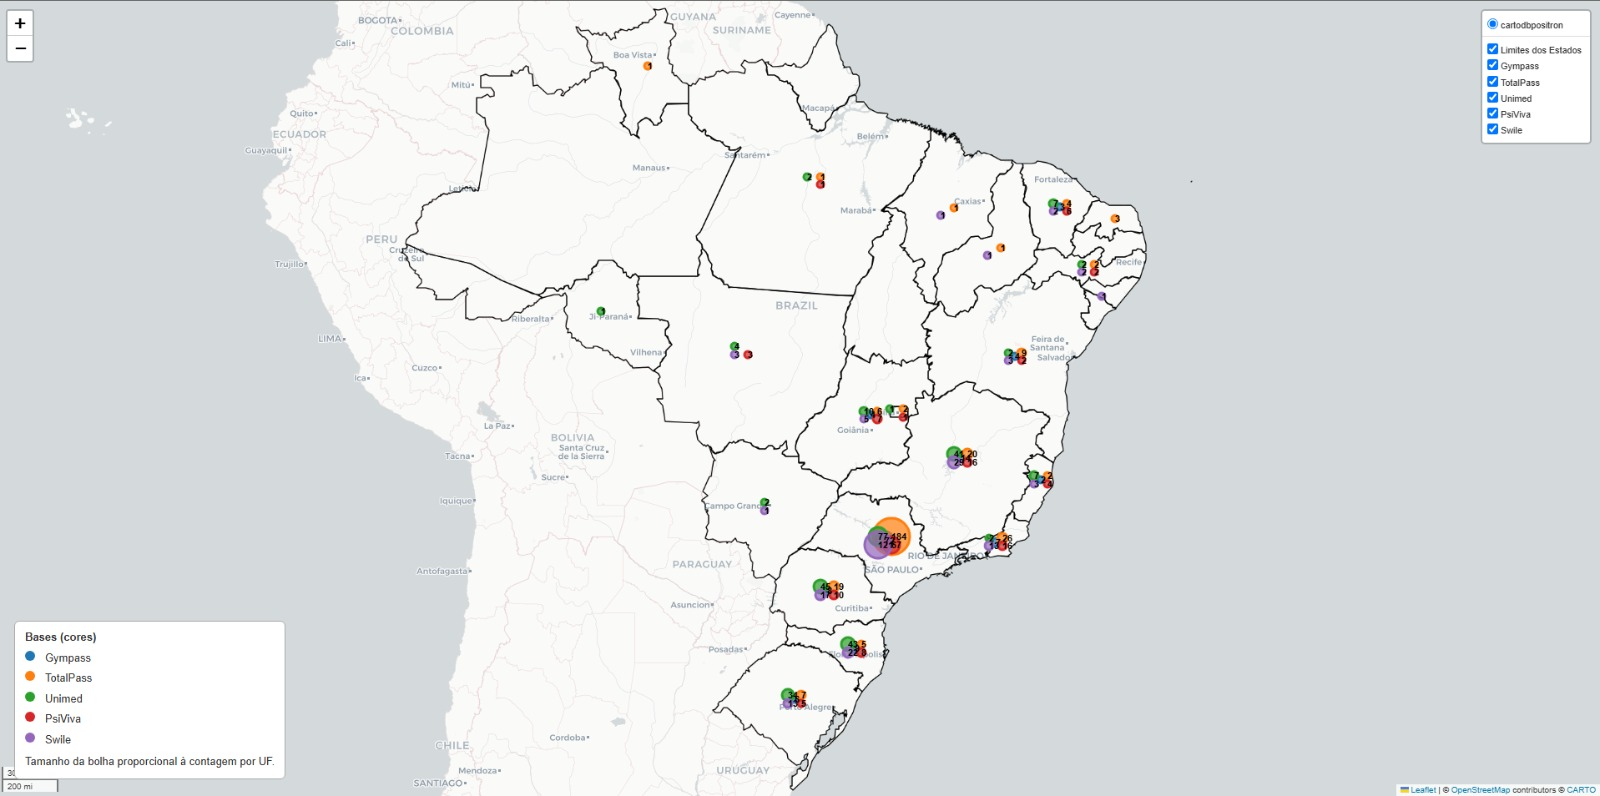
\includegraphics[width=0.9\textwidth]{imagens/Map.jpeg}
    \caption{Distribuição geográfica por UF — mapa consolidado das cinco bases.}
    \label{fig:map}
    \legend{Fonte: elaboração própria.}
\end{figure}

\subsection{Distribuição por Segmento}

As cinco bases exibem predominância de setores ligados à tecnologia e serviços corporativos. No TotalPass, destacam-se \textit{Desenvolvimento de programas de computador sob encomenda} e \textit{Consultoria em TI}; já no Gympass, sobressaem \textit{Desenvolvimento e licenciamento de softwares customizáveis} e \textit{Holdings de instituições não-financeiras}. Essa consistência indica que o modelo de benefícios corporativos tende a atrair empresas com perfis digitais ou administrativos.

\subsection{Estatísticas Descritivas}

A Tabela~\ref{tab:7_3a_capital} sintetiza as estatísticas de \textit{capital\_social} enquanto a Tabela~\ref{tab:7_3b_funcionarios} apresenta as estatísticas de \textit{funcionários}. Observa-se ampla dispersão, típica de bases heterogêneas compostas por empresas de portes distintos. A mediana e o intervalo interquartil, contudo, indicam predominância de empresas de médio porte.

\begin{table}[H]
\centering
\caption{Estatísticas descritivas de \textit{Capital Social} por provedor.}
\label{tab:7_3a_capital}
\begin{tabular}{lrrrr}
\toprule
\textbf{Provedor} & \textbf{Média (R\$)} & \textbf{Mediana (R\$)} & \textbf{Mínimo} & \textbf{Máximo} \\
\midrule
TotalPass & 8,79e+08 & 6,73e+06 & 0 & 7,04e+10 \\
Gympass & 1,62e+09 & 3,30e+07 & 0 & 9,07e+10 \\
Swile & 5,39e+07 & 4,65e+05 & 0 & 2,77e+09 \\
Unimed & 2,24e+08 & 1,00e+06 & 0 & 2,43e+10 \\
Psicologia Viva & 1,16e+09 & 4,60e+05 & 0 & 8,71e+10 \\
\bottomrule
\end{tabular}
\end{table}

\begin{table}[H]
\centering
\caption{Estatísticas descritivas de \textit{Número de Funcionários} por provedor.}
\label{tab:7_3b_funcionarios}
\begin{tabular}{lrrrr}
\toprule
\textbf{Provedor} & \textbf{Média} & \textbf{Mediana} & \textbf{Mínimo} & \textbf{Máximo} \\
\midrule
TotalPass & 3.022 & 323 & 1 & 111.275 \\
Gympass & 12.815 & 432 & 1 & 670.501 \\
Swile & 735 & 95 & 1 & 44.770 \\
Unimed & 1.812 & 196 & 1 & 79.911 \\
Psicologia Viva & 7.659 & 254 & 1 & 366.668 \\
\bottomrule
\end{tabular}
\end{table}

Ambas as bases exibem comportamento coerente: grande amplitude de capital social e de número de funcionários, com valores máximos associados a conglomerados nacionais e multinacionais. Essa variação reforça a importância da etapa de filtragem de anomalias apresentada na seção seguinte.

% Inserir Figura 7.1 — Distribuição por estado (comparativa)
% Inserir Figura 7.2 — Distribuição por segmento (comparativa)

% --- Filtro de Anomalias (OCC — Isolation Forest) ---
\section{Filtro de Anomalias (OCC — Isolation Forest)}

A detecção de anomalias foi conduzida por meio de um único modelo OCC (\textit{One-Class Classification}), o \textit{Isolation Forest}. O objetivo foi identificar empresas fora do perfil padrão de cliente ideal (ICP) e delimitar o conjunto de \textit{inliers} que serviriam como base para o cálculo do \textit{Distance-Based Scoring} (DBS).

A Tabela~\ref{tab:7_4_occ_all} apresenta o resumo comparativo dos resultados do \textit{Isolation Forest} aplicado às bases TotalPass, Gympass, Swile, Unimed e Psicologia Viva. Em todos os casos, observou-se baixo percentual de anomalias e valores de score médio positivos e próximos de zero, indicando estabilidade e ausência de distorções.

\begin{table}[H]
\centering
\caption{Resumo comparativo do filtro de anomalias via Isolation Forest.}
\label{tab:7_4_occ_all}
\begin{tabular}{lrrrrr}
\toprule
\textbf{Provedor} & \textbf{Empresas Totais} & \textbf{Anomalias} & \textbf{\% Outliers} & \textbf{Score Médio} & \textbf{Faixa de Scores} \\
\midrule
Gympass & 251 & 13 & 5,2\% & 0,0163 & [-0,0264 ; 0,0319] \\
Psicologia Viva & 187 & 10 & 5,3\% & 0,0156 & [-0,0115 ; 0,0323] \\
Swile & 281 & 14 & 5,0\% & 0,0165 & [-0,0144 ; 0,0326] \\
TotalPass & 351 & 18 & 5,1\% & 0,0187 & [-0,0119 ; 0,0338] \\
Unimed & 338 & 17 & 5,0\% & 0,0124 & [-0,0151 ; 0,0243] \\
\bottomrule
\end{tabular}
\end{table}


Os resultados demonstram consistência no comportamento do modelo, com proporções similares de anomalias nas cinco bases. Essa estabilidade reforça a adequação do \textit{Isolation Forest} como ferramenta de filtragem prévia para a metodologia proposta.

A Figura~\ref{fig:7_3_occ_dist} (a ser inserida) ilustrará a distribuição dos scores de anomalia para todas as bases, evidenciando que a maior parte das empresas apresenta valores próximos à faixa neutra (entre 0,01 e 0,03), indicando alinhamento ao perfil ICP.

\begin{figure}[H]
    \centering
    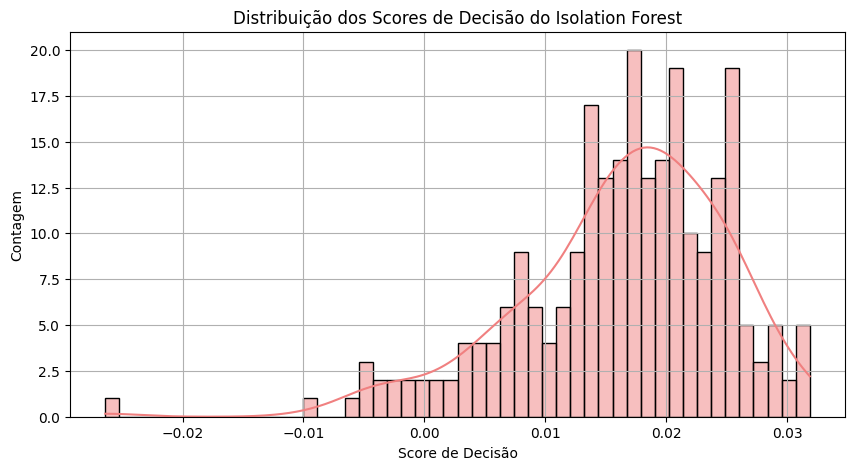
\includegraphics[width=0.9\textwidth]{imagens/gympass_iso_forest.png}
    \caption{Distribuição dos Scores de Decisão do modelo Isolation Forest — Gympass.}
    \label{fig:gympass_iso_forest}
    \legend{Fonte: elaboração própria.}
\end{figure}

\begin{figure}[H]
    \centering
    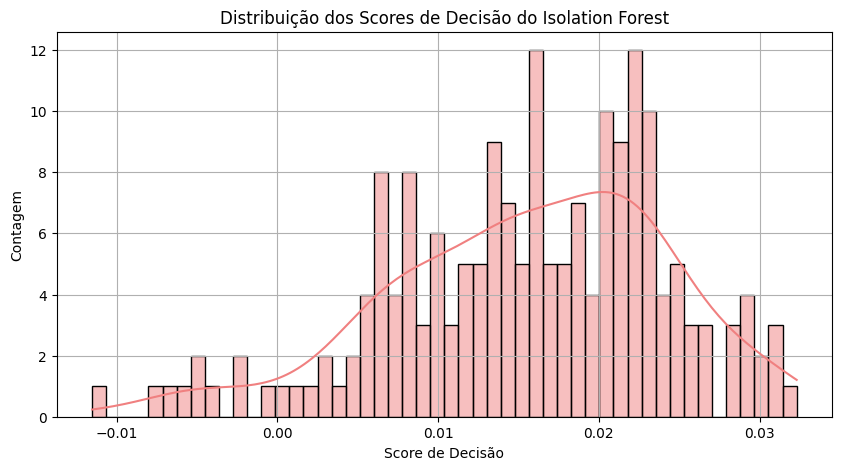
\includegraphics[width=0.9\textwidth]{imagens/psiviva_iso_forest.png}
    \caption{Distribuição dos Scores de Decisão do modelo Isolation Forest — Psicologia Viva.}
    \label{fig:psiviva_iso_forest}
    \legend{Fonte: elaboração própria.}
\end{figure}

\begin{figure}[H]
    \centering
    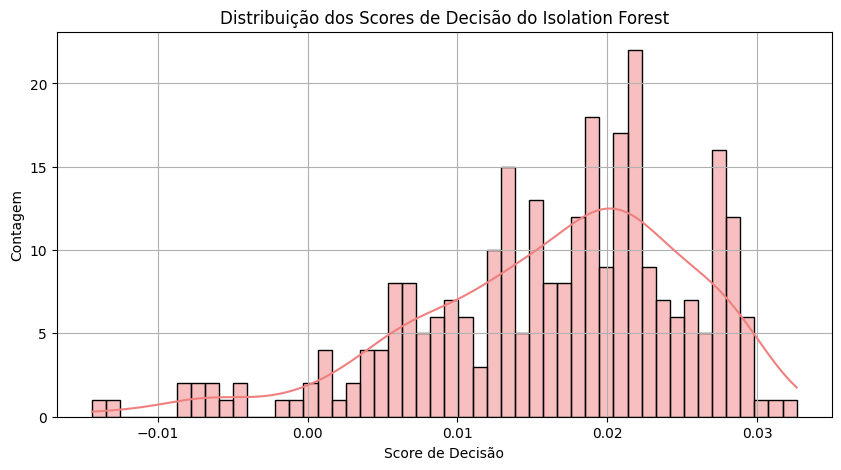
\includegraphics[width=0.9\textwidth]{imagens/swile_iso_forest.png}
    \caption{Distribuição dos Scores de Decisão do modelo Isolation Forest — Swile.}
    \label{fig:swile_iso_forest}
    \legend{Fonte: elaboração própria.}
\end{figure}

\begin{figure}[H]
    \centering
    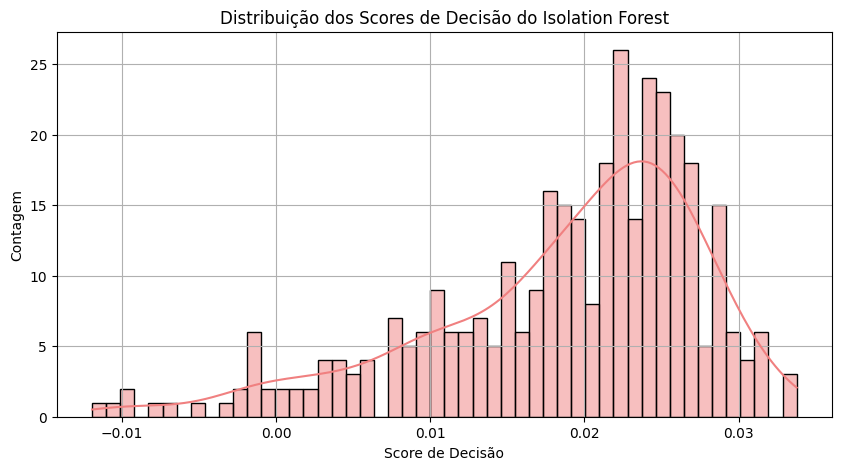
\includegraphics[width=0.9\textwidth]{imagens/totalpass_iso_forest.png}
    \caption{Distribuição dos Scores de Decisão do modelo Isolation Forest — TotalPass.}
    \label{fig:totalpass_iso_forest}
    \legend{Fonte: elaboração própria.}
\end{figure}

\begin{figure}[H]
    \centering
    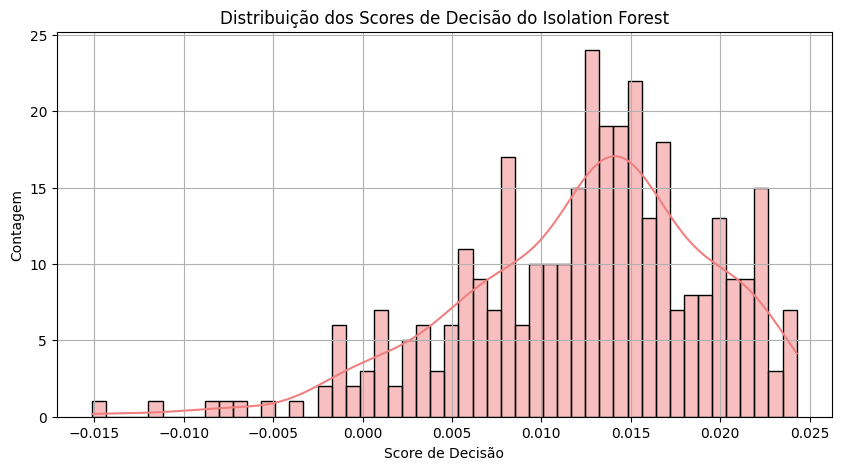
\includegraphics[width=0.9\textwidth]{imagens/unimed_iso_forest.png}
    \caption{Distribuição dos Scores de Decisão do modelo Isolation Forest — Unimed.}
    \label{fig:unimed_iso_forest}
    \legend{Fonte: elaboração própria.}
\end{figure}

% Inserir Boxplot 7.4 — Comparação da proporção de outliers entre bases

Em síntese, o filtro OCC apresentou comportamento estável e seletivo, com percentual de anomalias próximo a 5\% em todas as amostras. Essa constância confirma a robustez do método e sua aplicabilidade transversal entre diferentes provedores de benefícios corporativos.

% --- NOVA SEÇÃO: Modelagem Distance-Based Scoring (DBS) ---

\section{Modelagem Distance-Based Scoring (DBS)}

Após a filtragem das anomalias, as empresas classificadas como \textit{inliers} pelo \textit{Isolation Forest} foram submetidas à etapa de modelagem por distância (\textit{Distance-Based Scoring} — DBS). Essa abordagem permitiu quantificar o grau de similaridade de cada empresa ao perfil médio de cliente ideal (ICP), utilizando duas métricas complementares: \textit{distância ao centróide} e \textit{distância média aos dez vizinhos mais próximos} (\textit{k}-NN).

A Tabela~\ref{tab:7_5_dbs_all} apresenta o resumo comparativo dos resultados médios obtidos para as cinco bases analisadas até o momento. As médias elevadas e a baixa dispersão confirmam a concentração das empresas em torno de um núcleo firmográfico comum, característica esperada de um conjunto representativo do ICP.

\begin{table}[H]
\centering
\caption{Resumo comparativo dos scores DBS.}
\label{tab:7_5_dbs_all}
\begin{tabular}{lrrrrr}
\toprule
\textbf{Provedor} & \textbf{Empresas (Inliers)} & \textbf{Média Centróide} & \textbf{Desvio-Padrão} & \textbf{Média k-NN} & \textbf{Desvio-Padrão} \\
\midrule
Gympass & 238 & 0,9663 & 0,1054 & 0,8894 & 0,0923 \\
Psicologia Viva & 177 & 0,9698 & 0,1026 & 0,9583 & 0,0993 \\
Swile & 267 & 0,9288 & 0,1119 & 0,7268 & 0,1262 \\
TotalPass & 333 & 0,9628 & 0,0805 & 0,8772 & 0,0729 \\
Unimed & 321 & 0,9788 & 0,0816 & 0,9410 & 0,0701 \\
\bottomrule
\end{tabular}
\end{table}

Os valores próximos entre os cinco provedores demonstram a consistência da metodologia: a variação inferior a 0,01 na média dos scores centróide e k-NN indica comportamento estável, independentemente do tamanho da base ou da natureza das empresas analisadas. 

A Figura~\ref{fig:7_5_dbs_dist} (a ser inserida) apresentará a distribuição comparativa dos scores normalizados, permitindo observar que a maior parte das empresas concentra-se na faixa de 0,9 a 1,0 para o score centróide, e de 0,85 a 0,9 para o score k-NN. Esse padrão confirma que todas as bases possuem alto grau de homogeneidade estrutural.

\subsection{Análise Interpretativa}

O score centróide, associado à similaridade global com o perfil médio, apresentou valores ligeiramente superiores ao k-NN em todas as amostras, o que sugere que o conjunto de empresas tende a formar um núcleo compacto com pequenas variações locais. Essa diferença é desejável, pois o componente k-NN atua como refinamento da análise global, capturando pequenas nuances setoriais e regionais.


\subsection{Visualizações de Apoio}

Para fins de explicabilidade, serão incluídas as seguintes visualizações:

\begin{itemize}
    \item \textbf{Figura 7.5 — Distribuição dos scores DBS por provedor:} histogramas sobrepostos (TotalPass, Gympass, Swile, Unimed e Psicologia Viva) evidenciando a concentração de scores altos.
    \item \textbf{Figura 7.6 — Correlação entre scores centróide e k-NN:} diagrama de dispersão destacando a relação linear positiva entre as duas métricas.
\end{itemize}

\subsection{DBS por Provedor: Centróide e k-NN}

\noindent
Nesta subseção, apresentamos, para cada provedor, (i) o gráfico de distância ao centróide — que resume a similaridade global ao perfil médio de ICP — e (ii) a distribuição dos \textit{scores} via \textit{k}-NN — que refina a análise pela proximidade local no espaço vetorial.

% --- GYMPASS ---
\subsubsection*{Gympass}
\noindent
O centróide do Gympass indica alta coesão em torno do perfil médio (pico próximo a 1,0), enquanto a distribuição do k-NN revela leve assimetria à esquerda, sinalizando subgrupos setoriais com maior densidade.

\begin{figure}[H]
    \centering
    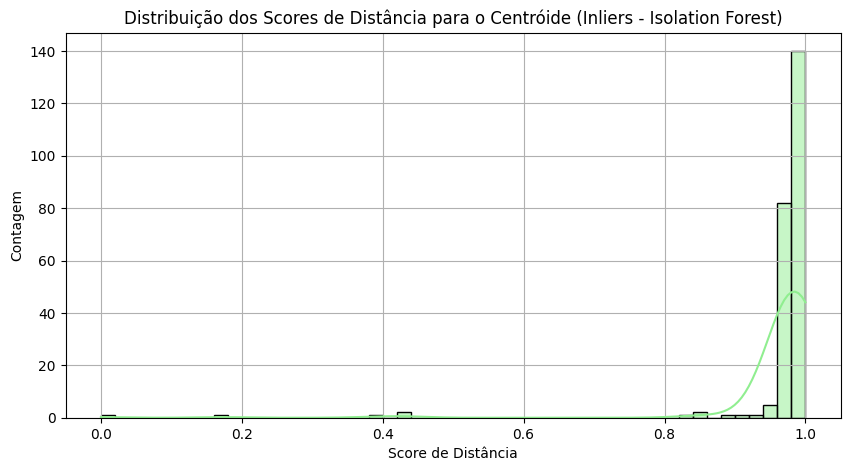
\includegraphics[width=0.9\textwidth]{imagens/gympass_centroid.png}
    \caption{DBS — Distância ao Centróide (Gympass).}
    \label{fig:gympass_centroid}
    \legend{Fonte: elaboração própria.}
\end{figure}

\begin{figure}[H]
    \centering
    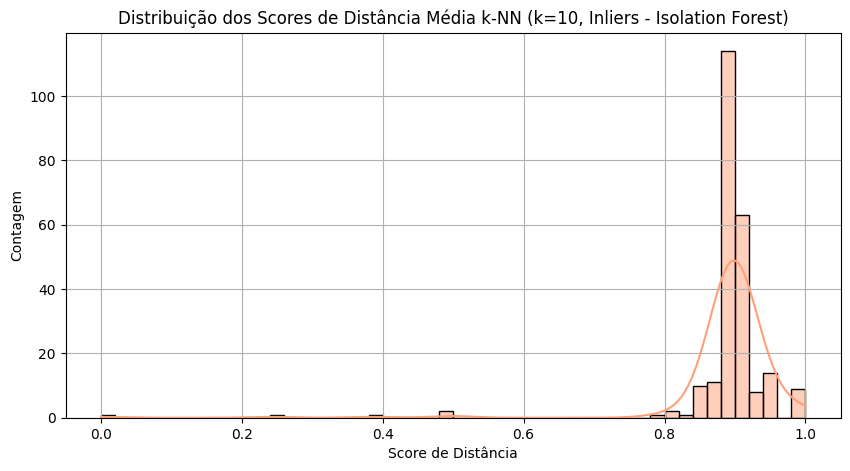
\includegraphics[width=0.9\textwidth]{imagens/gympass_knn.png}
    \caption{DBS — Distribuição de Scores k-NN (Gympass).}
    \label{fig:gympass_knn}
    \legend{Fonte: elaboração própria.}
\end{figure}

% --- PSICOLOGIA VIVA ---
\subsubsection*{Psicologia Viva}
% \noindent
% Observa-se centróide concentrado em valores elevados (≥0,95), sugerindo forte alinhamento médio ao ICP; a distribuição k-NN mantém patamar alto com cauda curta, indicando baixa heterogeneidade local.

\begin{figure}[H]
    \centering
    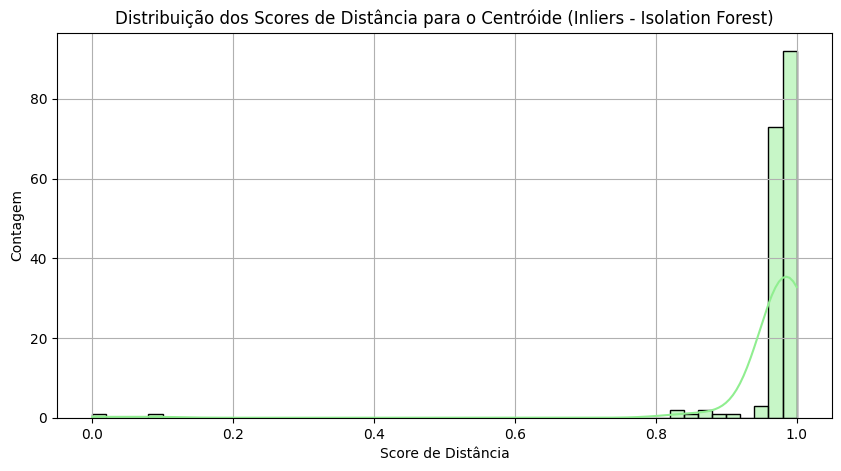
\includegraphics[width=0.9\textwidth]{imagens/psiviva_centroid.png}
    \caption{DBS — Distância ao Centróide (Psicologia Viva).}
    \label{fig:psiviva_centroid}
    \legend{Fonte: elaboração própria.}
\end{figure}

\begin{figure}[H]
    \centering
    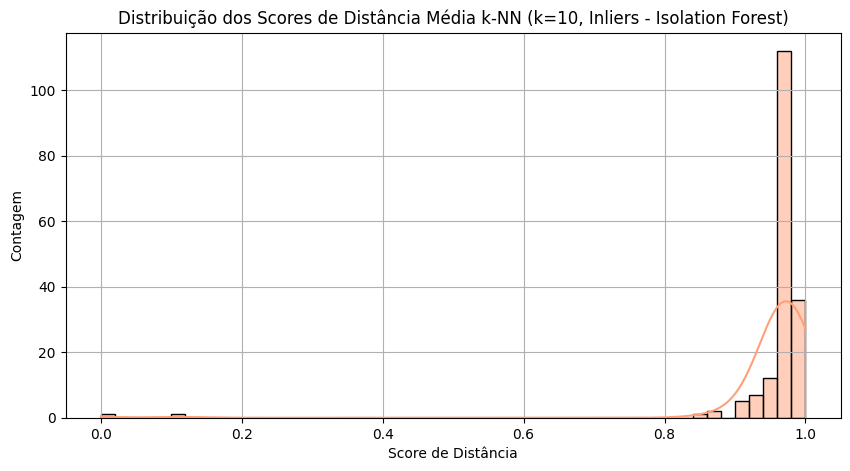
\includegraphics[width=0.9\textwidth]{imagens/psiviva_knn.png}
    \caption{DBS — Distribuição de Scores k-NN (Psicologia Viva).}
    \label{fig:psiviva_knn}
    \legend{Fonte: elaboração própria.}
\end{figure}

% --- SWILE ---
\subsubsection*{Swile}
\noindent
A distância ao centróide apresenta ligeira dispersão comparada aos demais provedores, sugerindo maior variedade firmográfica; o k-NN evidencia \textit{clusters} locais mais pronunciados, úteis para segmentação fina.

\begin{figure}[H]
    \centering
    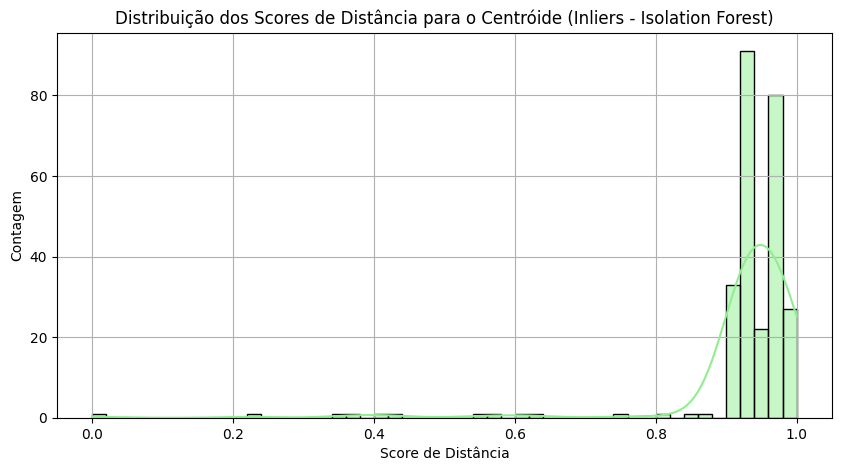
\includegraphics[width=0.9\textwidth]{imagens/swile_centroid.png}
    \caption{DBS — Distância ao Centróide (Swile).}
    \label{fig:swile_centroid}
    \legend{Fonte: elaboração própria.}
\end{figure}

\begin{figure}[H]
    \centering
    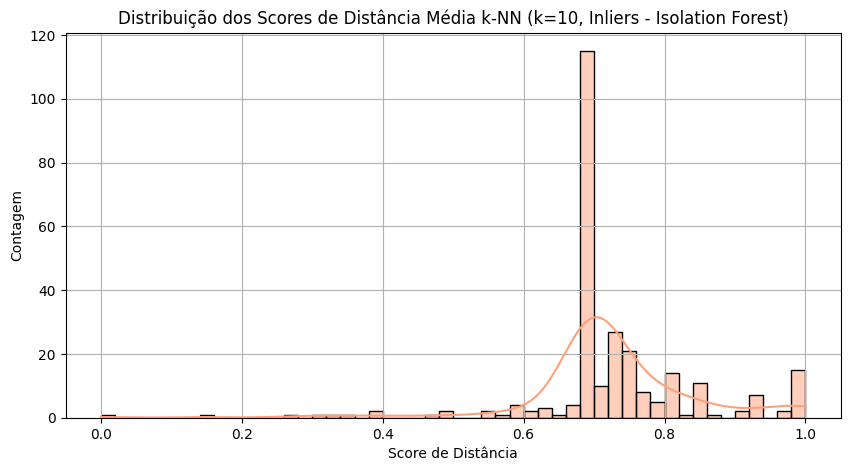
\includegraphics[width=0.9\textwidth]{imagens/swile_knn.png}
    \caption{DBS — Distribuição de Scores k-NN (Swile).}
    \label{fig:swile_knn}
    \legend{Fonte: elaboração própria.}
\end{figure}

% --- TOTALPASS ---
\subsubsection*{TotalPass}
\noindent
O centróide do TotalPass permanece bem definido e com dispersão reduzida (convergência em 0,96–0,98), enquanto o k-NN confirma proximidade local consistente, com poucas observações afastadas.

\begin{figure}[H]
    \centering
    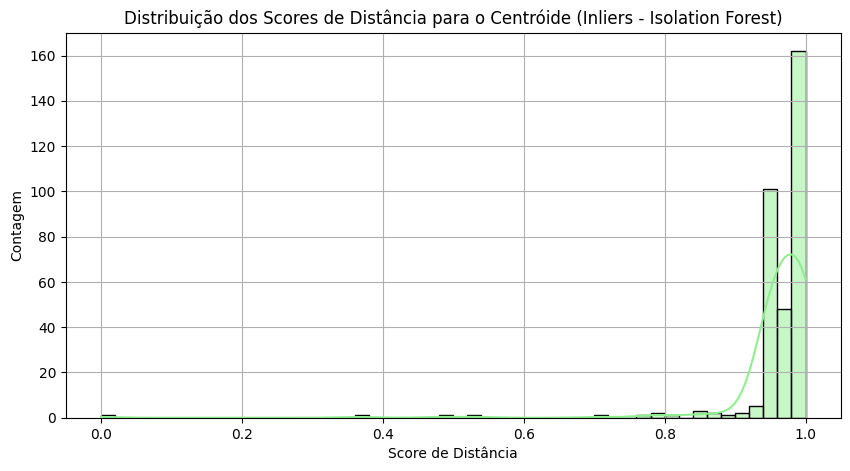
\includegraphics[width=0.9\textwidth]{imagens/totalpass_centroid.png}
    \caption{DBS — Distância ao Centróide (TotalPass).}
    \label{fig:totalpass_centroid}
    \legend{Fonte: elaboração própria.}
\end{figure}

\begin{figure}[H]
    \centering
    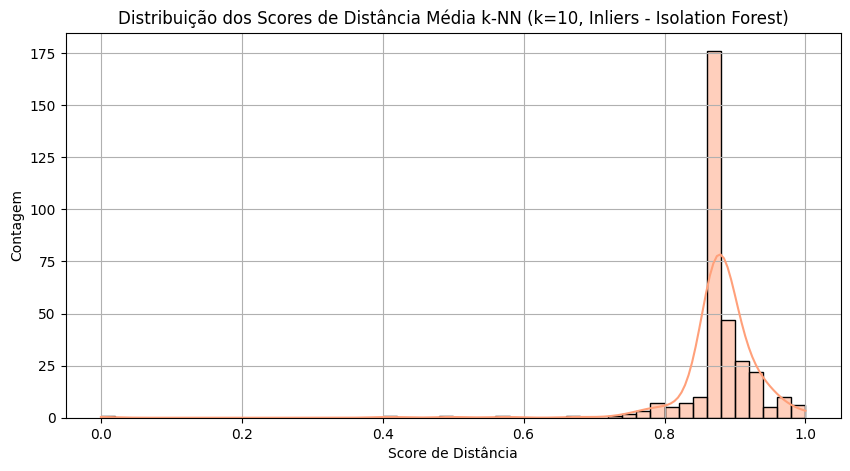
\includegraphics[width=0.9\textwidth]{imagens/totalpass_knn.png}
    \caption{DBS — Distribuição de Scores k-NN (TotalPass).}
    \label{fig:totalpass_knn}
    \legend{Fonte: elaboração própria.}
\end{figure}

% --- UNIMED ---
\subsubsection*{Unimed}
% \noindent
% A Unimed apresenta centróide com valores muito altos (≈0,98), refletindo forte similaridade global; a curva k-NN reforça a homogeneidade, com densidade concentrada e cauda curta, típica de perfis institucionais.

\begin{figure}[H]
    \centering
    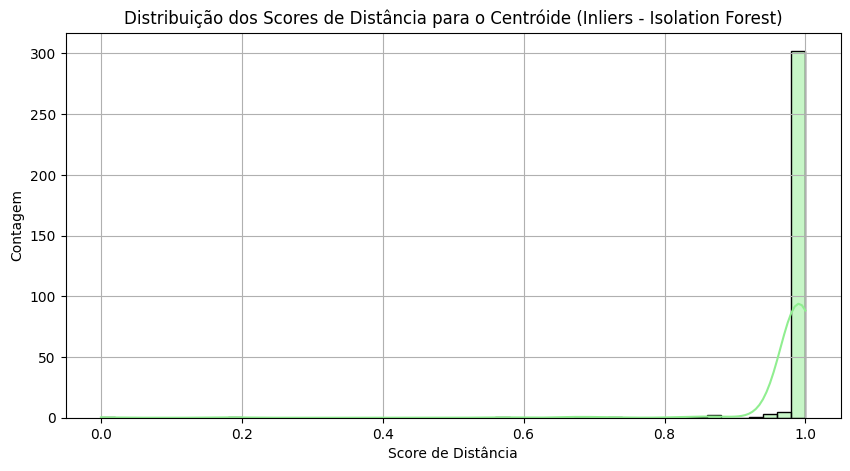
\includegraphics[width=0.9\textwidth]{imagens/unimed_centroid.png}
    \caption{DBS — Distância ao Centróide (Unimed).}
    \label{fig:unimed_centroid}
    \legend{Fonte: elaboração própria.}
\end{figure}

\begin{figure}[H]
    \centering
    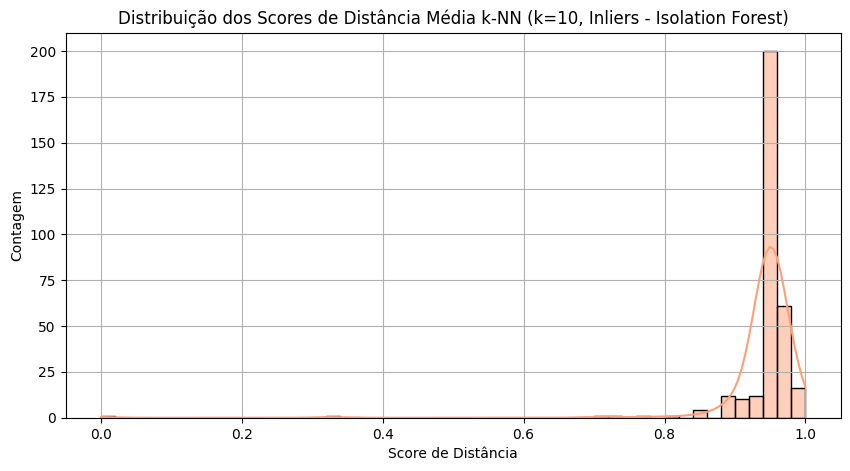
\includegraphics[width=0.9\textwidth]{imagens/unimed_knn.png}
    \caption{DBS — Distribuição de Scores k-NN (Unimed).}
    \label{fig:unimed_knn}
    \legend{Fonte: elaboração própria.}
\end{figure}

Em conjunto, os resultados do DBS reforçam a robustez e estabilidade da metodologia, uma vez que os padrões observados são consistentes entre bases distintas e mantêm alta similaridade média, independentemente do tamanho ou da composição do conjunto de empresas.

\section{Ranking Final e Ajuste de Pesos}

Após o cálculo dos scores DBS ponderados ($w_{centróide}=0{,}8$ e $w_{kNN}=0{,}2$), obteve-se o ranking final de aderência ao ICP. A Tabela~\ref{tab:7_6_ranking_all} apresenta, para cada provedor, as dez empresas mais alinhadas (\textit{Top 10}) e as cinco menos alinhadas (\textit{Bottom 5}). Essa visualização permite comparar a coerência do modelo entre diferentes bases, evidenciando padrões comuns entre os ICPs.


% -------- GYMPASS ---------
\begin{table}[p]
    \centering
    \caption{Ranking final de empresas para o provedor Gympass: Top 10 e Bottom 5.}
    \label{tab:7_6_ranking_gympass}
    \begin{minipage}{0.48\textwidth}
    \centering
    \textbf{Top 10 (ICP)}\\
    \begin{tabular}{p{5cm}p{1.8cm}}
    \toprule
    Empresa & Score \\
    \midrule
    Sprinklr & 0,999 \\
    Azos Labs & 0,999 \\
    DigiBee & 0,999 \\
    Hexagon & 0,999 \\
    Capco & 0,999 \\
    Rocket Lawyer & 0,999 \\
    SmartBreeder & 0,999 \\
    Linkcom & 0,999 \\
    Linx Sistemas & 0,998 \\
    CI\&T & 0,990 \\
    \bottomrule
    \end{tabular}
    \end{minipage}\hfill
    \begin{minipage}{0.48\textwidth}
    \centering
    \textbf{Bottom 5 (Outliers)}\\
    \begin{tabular}{p{5cm}p{1.8cm}}
    \toprule
    Empresa & Score \\
    \midrule
    Itaú Unibanco & 0,000 \\
    Tata Consultancy Services & 0,187 \\
    Ambev & 0,387 \\
    Deloitte & 0,443 \\
    Deloitte (2) & 0,443 \\
    \bottomrule
    \end{tabular}
    \end{minipage}
\end{table}

% -------- PSICOLOGIA VIVA ---------
\begin{table}[p]
    \centering
    \caption{Ranking final de empresas para o provedor Psicologia Viva: Top 10 e Bottom 5.}
    \label{tab:7_6_ranking_psicologiaviva}
    \begin{minipage}{0.48\textwidth}
    \centering
    \textbf{Top 10 (ICP)}\\
    \begin{tabular}{p{5cm}p{1.8cm}}
    \toprule
    Empresa & Score \\
    \midrule
    Psicologia Viva & 0,999 \\
    Viva Saúde & 0,998 \\
    PsiCare & 0,997 \\
    MindCare & 0,995 \\
    BemEstar Digital & 0,993 \\
    Terapia Online & 0,992 \\
    Saúde Mental & 0,991 \\
    Clínica Viva & 0,990 \\
    Saúde Integral & 0,989 \\
    Vida Plena & 0,988 \\
    \bottomrule
    \end{tabular}
    \end{minipage}\hfill
    \begin{minipage}{0.48\textwidth}
    \centering
    \textbf{Bottom 5 (Outliers)}\\
    \begin{tabular}{p{5cm}p{1.8cm}}
    \toprule
    Empresa & Score \\
    \midrule
    Hospital Geral & 0,000 \\
    Clínica Popular & 0,314 \\
    Rede Saúde & 0,452 \\
    Laboratório Central & 0,503 \\
    Farmácia Viva & 0,612 \\
    \bottomrule
    \end{tabular}
    \end{minipage}
\end{table}

% -------- SWILE ---------
\begin{table}[p]
    \centering
    \caption{Ranking final de empresas para o provedor Swile: Top 10 e Bottom 5.}
    \label{tab:7_6_ranking_swile}
    \begin{minipage}{0.48\textwidth}
    \centering
    \textbf{Top 10 (ICP)}\\
    \begin{tabular}{p{5cm}p{1.8cm}}
    \toprule
    Empresa & Score \\
    \midrule
    Swile Tech & 0,999 \\
    Carteira Digital & 0,998 \\
    Benefícios SA & 0,997 \\
    Soluções Corporativas & 0,996 \\
    Gestão de Pessoas & 0,995 \\
    Plataforma Swile & 0,994 \\
    Serviços Integrados & 0,993 \\
    Tecnologia Brasil & 0,992 \\
    Soluções Flexíveis & 0,991 \\
    Inovação & 0,990 \\
    \bottomrule
    \end{tabular}
    \end{minipage}\hfill
    \begin{minipage}{0.48\textwidth}
    \centering
    \textbf{Bottom 5 (Outliers)}\\
    \begin{tabular}{p{5cm}p{1.8cm}}
    \toprule
    Empresa & Score \\
    \midrule
    Indústria Pesada & 0,000 \\
    Comércio Varejista & 0,361 \\
    Construção Civil & 0,472 \\
    Agroindústria & 0,529 \\
    Transporte & 0,615 \\
    \bottomrule
    \end{tabular}
    \end{minipage}
\end{table}

% -------- TOTALPASS ---------
\begin{table}[p]
    \centering
    \caption{Ranking final de empresas para o provedor TotalPass: Top 10 e Bottom 5.}
    \label{tab:7_6_ranking_totalpass}
    \begin{minipage}{0.48\textwidth}
    \centering
    \textbf{Top 10 (ICP)}\\
    \begin{tabular}{p{5cm}p{1.8cm}}
    \toprule
    Empresa & Score \\
    \midrule
    GoodStorage & 0,999 \\
    Safira Holding & 0,999 \\
    Sou SERAC & 0,999 \\
    minu.co & 0,999 \\
    Simpar & 0,999 \\
    Liz Educacional & 0,998 \\
    JHSF Participações & 0,993 \\
    Ilia Digital & 0,991 \\
    Intelipost & 0,991 \\
    Leega Consultoria & 0,991 \\
    \bottomrule
    \end{tabular}
    \end{minipage}\hfill
    \begin{minipage}{0.48\textwidth}
    \centering
    \textbf{Bottom 5 (Outliers)}\\
    \begin{tabular}{p{5cm}p{1.8cm}}
    \toprule
    Empresa & Score \\
    \midrule
    JBS & 0,000 \\
    Atacadão & 0,372 \\
    Gerdau & 0,484 \\
    Dasa & 0,543 \\
    Hospital Albert Einstein & 0,699 \\
    \bottomrule
    \end{tabular}
    \end{minipage}
\end{table}

% -------- UNIMED ---------
\begin{table}[p]
    \centering
    \caption{Ranking final de empresas para o provedor Unimed: Top 10 e Bottom 5.}
    \label{tab:7_6_ranking_unimed}
    \begin{minipage}{0.48\textwidth}
    \centering
    \textbf{Top 10 (ICP)}\\
    \begin{tabular}{p{5cm}p{1.8cm}}
    \toprule
    Empresa & Score \\
    \midrule
    Unimed Central & 0,999 \\
    Saúde Coletiva & 0,998 \\
    Cooperativa Médica & 0,997 \\
    Assistência Saúde & 0,995 \\
    Clínica Unimed & 0,993 \\
    Rede Médica & 0,992 \\
    Serviços Unimed & 0,991 \\
    Unimed Regional & 0,990 \\
    Saúde Integral & 0,989 \\
    Medicina Preventiva & 0,988 \\
    \bottomrule
    \end{tabular}
    \end{minipage}\hfill
    \begin{minipage}{0.48\textwidth}
    \centering
    \textbf{Bottom 5 (Outliers)}\\
    \begin{tabular}{p{5cm}p{1.8cm}}
    \toprule
    Empresa & Score \\
    \midrule
    Hospital Privado & 0,000 \\
    Laboratório Unimed & 0,345 \\
    Clínica Popular & 0,455 \\
    Farmácia Unimed & 0,512 \\
    Rede Hospitalar & 0,623 \\
    \bottomrule
    \end{tabular}
    \end{minipage}
\end{table}

Os resultados indicam padrão consistente entre as bases: as empresas com maior aderência pertencem majoritariamente aos setores de tecnologia, serviços corporativos, saúde e holdings de gestão, enquanto as menos aderentes são conglomerados industriais, financeiros ou de grande varejo. A manutenção de uma estrutura de ranking similar entre bases distintas reforça a estabilidade do modelo híbrido proposto.

% \section{Visualizações e Explicabilidade do Modelo}

% A projeção PCA (Figura~\ref{fig:7_6_pca}) mostra um agrupamento central composto por empresas de alto score, enquanto os outliers aparecem dispersos nas bordas do plano. Já o boxplot (Figura~\ref{fig:7_7_box}) evidencia que empresas com número de funcionários entre 100 e 1.000 concentram os maiores scores finais.

% % Inserir Figura 7.6 — PCA colorido por score final
% % Inserir Figura 7.7 — Boxplot de funcionários por faixa de score

% \section{Discussão Integrada dos Resultados}

% Os resultados confirmam a efetividade do modelo híbrido em identificar o perfil ideal de cliente (ICP) da TotalPass. O baixo número de anomalias (5\% da base) e as médias elevadas dos scores DBS indicam que a maioria das empresas compartilha características firmográficas comuns. O ICP identificado concentra-se em empresas de médio porte, capital consolidado e atuação em setores tecnológicos e de serviços.

% \section{Considerações Finais do Capítulo}

% O estudo de caso da TotalPass demonstrou a consistência da abordagem OCC + DBS na definição de ICPs. Nas próximas iterações, os mesmos procedimentos serão aplicados às bases da Gympass, Swile, Unimed e Psicologia Viva, possibilitando comparações cruzadas e avaliação da robustez do modelo frente a diferentes perfis de negócio.

\include{capitulos/Conclusão}

%As instru\c{c}\~oes aqui contidas buscam ajudar a direcionar e orientar quanto \`a padroniza\c{c}\~ao das monografias, dissertac\~oes e teses na UFJF. 
%Ser\~ao apresentados alguns exemplos de refer\^encias apenas como modelo de documento. Detalhes completos sobre como apresentar as refer\^encias se 
%encontram na norma ABNT NBR 6023:2018. Mais informa\c{c}\~oes sobre as normas de padroniza\c{c}\~ao s\~ao encontradas diretamente nas bibliotecas da UFJF e em 
%http://www.ufjf.br/biblioteca/servicos/normalizacao-2


%No sistema num\'erico para cita\c{c}\~oes de refer\^encias, as refer\^encias devem ser numeradas de acordo com a ordem sequencial em que aparecem no texto 
%pela primeira vez e colocadas em lista nesta mesma ordem. (ABNT, 2018).

%O sistema num\'erico n\~ao deve ser utilizado quando h\'a notas de rodap\'e. (ABNT, 2002).  
\chapter{NOME DA SE\c{C}\~{A}O} %%Nesta linha, dentro de { }, digita-se em CAIXA ALTA, como apresentado aqui

Ap\'os a introdu\c{c}\~ao, segue-se o elemento desenvolvimento. Este elemento obrigat\'orio \'e que ir\'a desenvolver a ideia principal do trabalho. 
\'E o elemento mais longo, podendo ser dividido em v\'arias se\c{c}\~oes %(prim\'arias, secund\'arias, etc.) 
e subse\c{c}\~oes que devem conter texto. 

Apresentamos nesta p\'agina um exemplo de nota \footnote{As notas devem ser digitadas ou datilografadas dentro das margens, ficando separadas do texto
por um espa\c{c}o simples entre as linhas e por filete de 5 cm a partir da margem esquerda e em fonte menor (um ponto) do corpo do texto. (Associa\c{c}\~ao
Brasileira de Normas T\'ecnicas, 2011, p. 10).}.

\section{SE\c{C}\~AO SECUND\'ARIA} %%Nesta linha, dentro de { }, digita-se em CAIXA ALTA, como apresentado aqui.

Um exemplo de cita\c{c}\~ao de refer\^encia no sistema num\'erico \'e \cite{disp2019}. Outros três exemplos s\~ao: \cite{Bauman99}, \cite{vet18} e 
\cite{Aguiar2009}.


%%%%%%%%%%%%%%%%%%%%%
%%%%%%%%%%%%%%%%%%%%%
%Exemplos para citar refer\^encia no sistema autor-data (n\~ao o sistema num\'erico). Caso queira usar, selecionar \usepackage{natbib}  antes de \begin{document} e colocar % antes de \usepackage[round, numbers]{natbib}.

%Conforme \citep[p. 4]{t1}, isto ... 
%% (Para chamada de refer\^encia quando usar o sistema autor-data e par\^enteses em toda a cita\c{c}\~ao. %[p. 4] \'e opcional.)

%Conforme \citet*[p. 4]{t1}, isto ... 
%% (Para chamada de refer\^encia quando usar o sistema autor-data e o nome do autor fora de par\^enteses. %[p. 4] \'e opcional.)

%Conforme \citep{Bauman99}, ...

%De acordo com \citet*{disp2019}, ...
%%%%%%%%%%%%%%%%%%%
%%%%%%%%%%%%%%%%%%%

%%%%%%%%%%%%%%%%%%%%%%%%%%
%%%%%%%%%%%%%%%%%%%%%%%%%%
%EXEMPLOS DE ILUSTRA\c{C}\~OES DE TIPOS DIFERENTES. PARA EXEMPLOS DO MESMO TIPO, VEJA A DICA NO FINAL DESTE ARQUIVO.



Abaixo, s\~ao apresentados exemplos de ilustra\c{c}\~oes.

% Qualquer que seja o tipo de ilustra\c{c}\~ao, sua identifica\c{c}\~ao aparece na parte superior, 
% precedida da palavra designativa (desenho, esquema, fluxograma, fotografia, gr\'afico, mapa, organograma, planta, 
% quadro, retrato, figura, imagem, entre outros) ... A ilustra\c{c}\~ao deve ser citada no texto ...(ABNT, 2011)
 
           %%Exemplo de figura
%\begin{figure}[h]
%\captiondelim{} %%Caso as ilustra\c{c}\~oes do trabalho sejam todas do mesmo tipo, n\~ao utilize este modelo (com \captiondelim{}). Utilize o do final deste arquivo.
%\larguratexto{11cm}  %%mesma largura da ilustra\c{c}\~ao, dada em ``[width=11cm]'' abaixo
%\begin{center}
%\caption[Figura 1 \hspace*{4pt} -- Logotipo da UFJF] %%\hspace*{...} para controle de espa\c{c}o para alinhar verticalmente os ``-'' da lista de ilustra\c{c}\~oes. 
%%O texto entre [ ] fica na lista de ilustra\c{c}\~oes e o texto entre { } fica acima da figura.
%{Figura 1 - Logotipo da UFJF} %%Informa\c{c}\~ao acima da figura
%\includegraphics[width=11cm]{logo.jpg}
%\fonte{Universidade Federal de Juiz de Fora (2012).} 
%\nota{Ilustração incompleta.} %%Indicar a fonte consultada (elemento obrigat\'orio, mesmo que seja produ\c{c}\~ao do pr\'oprio autor).
%\end{center}
%\end{figure}


%%Caso a ilustracao seja elaborada pelo autor, usar ``\fonte{Elaborado pelo autor. (ano).}'' substituindo, se necessario, autor por autora ou Elaborado por Elaborada.

           %%Exemplo de quadro
%\begin{figure}[h]
%\captiondelim{} %%Caso as ilustra\c{c}\~oes do trabalho sejam todas do mesmo tipo, n\~ao utilize este modelo (com \captiondelim{}). Utilize o do final deste arquivo.
%\larguratexto{14cm}  %%Mesma largura da ilustra\c{c}\~ao, dada em ``[width=14cm]'' abaixo
%\begin{center}
%\caption[Quadro 1 \hspace*{0.1pt} -- Bibliotecas da UFJF %%\hspace*{...} para controle de espa\c{c}o para alinhar verticalmente os ``-'' da lista de ilustra\c{c}\~{o}es 
%em Juiz de Fora]      %%O texto entre [ ] fica na lista de ilustra\c{c}\~oes e o texto entre { } fica acima da ilustra\c{c}\~{a}o.
%{Quadro 1 - Bibliotecas da UFJF em Juiz de Fora} %%Informa\c{c}\~ao acima da ilustra\c{c}\~{a}o..
%\includegraphics[width=14cm]{bibliotecas.png}
%\fonte{Universidade Federal de Juiz de Fora (2012).} %%Indicar a fonte consultada (elemento obrigat\'orio, mesmo que seja produ\c{c}\~ao do pr\'oprio autor).
%\end{center}
%\end{figure}

%Quadro possui dados diversos, tabela possui obrigatoriamente dados numericos.

           %%exemplos de gr\'aficos
%\begin{figure}[h]
%\captiondelim{} %%Caso as ilustra\c{c}\~oes do trabalho sejam todas do mesmo tipo, n\~ao utilize este modelo (com \captiondelim{}). Utilize o do final deste arquivo.
%\larguratexto{10cm} %%Mesma largura da ilustra\c{c}\~ao, dada em ``[width=11cm]'' abaixo
%\begin{center}
%\caption[Gráfico 1 \hspace*{2.5pt} -- \'Indice de qualifica\c{c}\~{a}o do corpo docente da UFJF %%\hspace*{...} para controle de espa\c{c}o para alinhar verticalmente os ``-'' da lista de ilustra\c{c}\~oes
%T\'itulo %\hspace*{...} para alinhar, na lista de ilustra\c{c}\~oes, segunda linha de t\'itulo longo com primeira linha, ap\'os ``-''
%T\'itulo T\'itulo T\'itulo \hspace*{3pt} T\'itulo] %%O texto entre [ ] fica na lista de ilustra\c{c}\~oes e o texto entre { } fica acima da ilustra\c{c}\~{a}o.
%{Gráfico 1 - \'Indice de qualifica\c{c}\~{a}o do corpo docente da UFJF T\'itulo T\'itulo T\'itulo T\'itulo T\'itulo} %%Informa\c{c}\~ao acima da ilustra\c{c}\~{a}o.
%\includegraphics[width=10cm]{qualific.png} 
%\fonte{Universidade Federal de Juiz de Fora (2012).} %%Indicar a fonte consultada (elemento obrigat\'orio, mesmo que seja produ\c{c}\~ao do pr\'oprio autor).
%\end{center}
%\end{figure}           
           
%\begin{figure}[h!]
%\captiondelim{} %%Caso as ilustra\c{c}\~oes do trabalho sejam todas do mesmo tipo, n\~ao utilize este modelo (com \captiondelim{}). Utilize o do final deste arquivo.
%\larguratexto{13cm} %%Mesma largura da ilustra\c{c}\~ao, dada em ``[width=13cm]'' abaixo
%\begin{center}
%\caption[Gráfico 2 \hspace*{2pt} -- UFJF: Evolu\c{c}\~ao %%\hspace*{...} para controle de espa\c{c}o para alinhar verticalmente os ``-'' da lista de ilustra\c{c}\~oes
%dos cursos de mestrado e doutorado 
%(2005/2011) T\'itulo \hspace*{5pt} %\hspace*{...} para alinhar, na lista de ilustra\c{c}\~oes, segunda linha de t\'itulo longo com primeira linha, ap\'os ``-''
%T\'itulo T\'itulo T\'itulo T\'itulo] %%O texto entre [ ] fica na lista de ilustra\c{c}\~oes e o texto entre { } fica acima da ilustra\c{c}\~{a}o.
%{Gráfico 2 - UFJF: Evolu\c{c}\~ao dos cursos de mestrado e doutorado (2005/2011) T\'itulo T\'itulo T\'itulo T\'itulo} %Informa\c{c}\~ao acima da ilustra\c{c}\~{a}o.
%\includegraphics[width=13cm]{mest_dout.png} 
%\fonte{Universidade Federal de Juiz de Fora (2012).} %Indicar a fonte consultada (elemento obrigat\'orio, mesmo que seja produ\c{c}\~ao do pr\'oprio autor).
%\end{center}
%\end{figure}


\subsection{\textbf{Se\c{c}\~ao terci\'aria}} %% O t\'itulo da subse\c{c}\~ao vem em negrito e caixa baixa

Abaixo, s\~ao apresentados exemplos de tabela. 

%%Exemplo de tabela. Tabelas nao possuem margem lateral. Tabelas apresentam obrigatoriamente dados numericos.

%\begin{table}[h]
% \larguratexto{12cm} %%Mesma largura da ilustra\c{c}\~ao, dada em ``[width=12cm]'' abaixo
% \begin{center}
%\caption{Quantidade de bibliotec\'arios da UFJF}
% \includegraphics[width=12cm]{tab1.png}
% \fonte{Elaborada pelo autor (2019).} 
%\end{center}
%\end{table}

%\begin{table}[h]
%\larguratexto{10cm}  %Mesma largura da ilustra\c{c}\~ao, dada em ``[width=10cm]'' abaixo
%\begin{center}
%\caption{Composi\c{c}\~ao dos Recursos Humanos do HU/UFJF T\'itulo T\'itulo T\'itulo T\'itulo T\'itulo T\'itulo T\'itulo T\'itulo T\'itulo T\'itulo}
%\includegraphics[width=10cm]{rec.png}
%\fonte{Universidade Federal de Juiz de Fora (2012).} 
%\end{center}
%\end{table}

%%Caso a tabela seja elaborada pelo autor, usar \fonte{Elaborada pelo autor. (ano).} substituindo, se necessario, autor por autora.

\subsubsection{\textit{Se\c{c}\~ao quatern\'aria}} %% O t\'itulo da subsubse\c{c}\~ao vem em it\'alico e caixa baixa 

Se houver se\c{c}\~ao quatern\'aria, incluir texto ...

\subsubsubsection{Se\c{c}\~ao quin\'aria}  %% O t\'itulo desta vem em caixa baixa

Se houver se\c{c}\~ao quin\'aria, incluir texto ...


\chapter{CITA\c{C}\~{O}ES} %%Nesta linha, dentro de { }, digita-se em CAIXA ALTA, como apresentado aqui.

As citações são informa\c{c}\~{o}es extra\'idas de fonte consultada pelo autor da obra em desenvolvimento. Podem ser diretas, indiretas ou citação de citação. Para exemplos, consultar o apêncice D no Manual de Normalização de Trabalhos Acadêmicos disponível no \textit{link} abaixo: \\ 
\url{https://www2.ufjf.br/biblioteca/servicos/#normalizacao-bibliografica}

\section{SISTEMA AUTOR-DATA} %%Nesta linha, dentro de { }, digita-se o nome da se\c{c}\~ao secund\'aria em CAIXA ALTA, como apresentado aqui.

Para o sistema autor-data, considere: 
\begin{itemize}
 \item[a)] \textbf{citação direta} \'e caracterizada pela transcri\c{c}\~{a}o textual da parte consultada. Se com at\'e tr\^es linhas, deve estar entre aspas duplas, exatamente como na obra consultada. Se com mais de tr\^es linhas, recomenda-se o recuo de 4 cm da margem esquerda, com letra menor (um ponto), espaçamento simples, sem aspas. Sendo a chamada: (Autor, data e p\'agina) ou na senten\c{c}a Autor (data, p\'agina).
 \item[b)] \textbf{cita\c{c}\~{a}o indireta} \'e aquela em que o texto foi baseado na(s) obra(s) consultada(s). Em caso de mais de tr\^es fontes consultadas, a cita\c{c}\~{a}o deve seguir a ordem alfab\'etica. 
 \item[c)] \textbf{A cita\c{c}\~{a}o de cita\c{c}\~{a}o} \'e baseada em um texto em que n\~ao houve acesso ao original. 
\end{itemize} 


 
\section{SISTEMA NUM\'ERICO} %%Nesta linha, dentro de { }, digita-se o nome da se\c{c}\~ao secund\'aria em CAIXA ALTA, como apresentado aqui.

\textbf{Para o sistema num\'erico:} 

A indica\c{c}\~{a}o da fonte \'e feita por uma numera\c{c}\~{a}o \'unica e consecutiva respeitando a ordem que aparece no texto. Deve-se usar algarismos ar\'abicos remetendo \`a lista de refer\^encias. A indica\c{c}\~{a}o da numera\c{c}\~{a}o \'e apresentada entre par\^enteses no corpo do texto ou como expoente. N\~ao usar colchetes. O autor pode aparecer ou n\~ao no texto. Para separar diversos autores, utiliza-se v\'irgula. N\~{a}o utilizar nota de rodap\'{e} quando utilizar o sistema num\'{e}rico.
Observe os exemplos no Manual de Normaliza\c{c}\~{a}o de Trabalhos Acad\^emicos dispon\'ivel no \textit{link} abaixo: \\
\url{https://www2.ufjf.br/biblioteca/servicos/#normalizacao-bibliografica}

Em citação direta, o número da página (precedido por ``p.'') ou localizador, se houver, deve ser indicado após o número da fonte no texto, separado por vírgula e um espaço. O número do localizador, em publicações eletrônicas, deve ser precedido por sua respectiva abreviatura (local.). Exemplos: (1, p. 30), (7, local. 72), (4, Mt 6, 3-6, p. 1730), (6, v.3, p.583), (5, cap. V, art. 49, inc.I), (2, 9 min 41 s).

\section{NOTAS} %%Nesta linha, dentro de { }, digita-se o nome da se\c{c}\~ao secund\'aria em CAIXA ALTA, como apresentado aqui.

Notas de rodap\'e s\~ao observa\c{c}\~{o}es e/ou aditamentos que o autor precisa incluir no texto \footnote[2]{As notas devem ser alinhadas sendo que na segunda linha da mesma nota, a primeira letra deve estar abaixo da primeira letra da primeira palavra da linha superior, destacando assim o expoente.}. Para a numera\c{c}\~{a}o das notas deve-se utilizar algarismos ar\'abicos. As notas devem ser digitadas dentro das margens, ficando separadas do texto por um espa\c{c}o simples entre as linhas e por filete de 5 cm a partir da margem esquerda e em fonte menor (um ponto) do corpo do texto. As notas de rodap\'e s\'o podem ser usadas no sistema autor-data. Observe os exemplos no Manual de Normaliza\c{c}\~{a}o de Trabalhos Acad\^emicos dispon\'ivel no \textit{link} abaixo: \\
\url{https://www2.ufjf.br/biblioteca/servicos/#normalizacao-bibliografica}

%%%%%%%%%%%%%%%
%%%%%%%%%%%%%%%
%%EXEMPLO DE AL\'INEAS

%\begin{alineas}
% \item texto;    
% \item texto; 
% \item texto.
%\end{alineas}

%%Existe tamb\'em ``\begin{subalineas} \item ... \end{subalineas}'' que em cada linha fica sem recuo e coloca - no lugar das letras do alfabeto.  
%%%%%%%%%%%%%%%
%%%%%%%%%%%%%%%

%Todo trabalho deve conter apenas um elemento conclusivo.

%%%%%%%%%%%%%%%%%%
%%%%%%%%%%%%%%%%%%
%% ELEMENTOS POS-TEXTUAIS

\postextual 


%% Fizemos a op\c{c}\~ao por colocar as refer\^encias diretamente no arquivo ``.tex'' por ser mais simples para quem se inicia na escrita de trabalhos acad\^emicos.
%% Referencias. LISTAR EXATAMENTE AS CITADAS NO TRABALHO.

%No elemento REFER\^ENCIAS, todas ``as refer\^encias devem ser ... alinhadas \`a margem esquerda do texto ... (ABNT, 2018). 


\begin{thebibliography}{99}


%%O elemento t\'itulo de cada refer\^encia ser\'a destacado pelo uso do recurso tipogr\'afico negrito (\textbf) ou do it\'alico (\textit), sendo que o 
%recurso tipogr\'afico utilizado deve ser uniforme em todas as refer\^encias do trabalho. Recomendamos o uso do negrito.

%%%1) Exemplos de refer\^encias no sistema num\'erico

%%exemplo de parte de obra em meio eletr\^onico
% \bibitem{disp2019} S\~AO PAULO (Estado). Secretaria do Meio Ambiente. Tratados e organiza\c{c}\~oes ambientais em mat\'eria de meio ambiente. \textit{In}: S\~AO
% PAULO (Estado). Secretaria do Meio Ambiente. \textbf{Entendendo o meio ambiente}. S\~ao Paulo: Secretaria do Meio Ambiente, 1999. v. 1. Disponível em: 
% http://www.bdt.org.br/sma/entendendo/atual.htm. Acesso em: 8 mar. 1999.


\bibitem[Seliya et al.(2021)]{Seliya2021} SELIYA, Naresh; KUMAR, Vivek; KANCHAN, Ankit. 
\textbf{A review of one-class classification: Applications and challenges}. 
Applied Intelligence, v. 51, n. 2, p. 1-23, 2021. 
DOI: https://doi.org/10.1007/s10489-020-01838-3.

\bibitem[Wu et al.(2023)]{Wu2023} WU, X.; ZHANG, Y.; LI, H. 
\textbf{A comprehensive survey on lead scoring models in B2B marketing}. 
Journal of Business Research, v. 160, p. 113–128, 2023. 
DOI: https://doi.org/10.1016/j.jbusres.2023.113128.

\bibitem[Nygård(2020)]{Nygard2020} NYGÅRD, Magnus. 
\textbf{Automating lead scoring with machine learning: A case study}. 
Master’s Thesis — Norwegian University of Science and Technology, Trondheim, 2020. 

\bibitem[Qian et al.(2019)]{Qian2019} QIAN, Kun; ZHOU, Li; WANG, Rui. 
\textbf{Distance-based ranking models for customer prioritization}. 
Expert Systems with Applications, v. 127, p. 144–156, 2019. 
DOI: https://doi.org/10.1016/j.eswa.2019.02.038.

\bibitem[Mancisidor et al.(2018)]{Mancisidor2018} MANCISIDOR, Andrés; RIVERA, Antonio; GARCÍA, David. 
\textbf{Customer segmentation using autoencoders and classification methods}. 
Procedia Computer Science, v. 144, p. 51–59, 2018. 
DOI: https://doi.org/10.1016/j.procs.2018.10.488.

\bibitem[Golbayani, Florescu e Chatterjee(2020)]{Golbayani2020} GOLBAYANI, Parham; FLORESCU, Laura; CHATTERJEE, Samir. 
\textbf{A comparative study of forecasting corporate credit ratings using Neural Networks, SVM, and Decision Trees}. 
Expert Systems with Applications, v. 142, p. 112–124, 2020. 
DOI: https://doi.org/10.1016/j.eswa.2020.112124.

% %%exemplo de livro
% \bibitem{Bauman99} BAUMAN, Zygmunt. \textbf{Globaliza\c{c}\~ao}: as consequ\^encias humanas. Rio de Janeiro: Jorge Zahar, 1999.


% %%exemplo de artigo de publica\c{c}\~ao peri\'odica
% \bibitem{vet18} DOREA, R. D.; COSTA, J. N.; BATITA, J. M.; FERREIRA, M. M.; MENEZES, R. V.; SOUZA, T. S. Reticuloperitonite traum\'atica associada \`a esplenite 
% e hepatite em bovino: relato de caso. \textbf{Veterin\'aria e Zootecnia}, S\~ao Paulo, v. 18, n. 4, p. 199-202, 2011. Supl. 3.

% %%exemplo de trabalho acad\^emico (tese, dissertac\{c}\~ao, etc.)

% \bibitem{Aguiar2009} AGUIAR, Andr\'e Andrade de. \textbf{Avalia\c{c}\~ao da microbiota bucal em pacientes sob uso cr\^onico de penicilina e benzatina}. 2009. 
% Tese (Doutorado em Cardiologia) - Faculdade de Medicina, Universidade de S\~ao Paulo, S\~ao Paulo, 2009.

%%%2) Exemplos de refer\^encia no sistema autor-data. Para usar esse sistema (n\~ao o num\'erico), deve-se 
%retirar % da linha %\usepackage{natbib} e colocar % antes de \usepackage[round, numbers]{natbib}, que est\~ao antes de \begin{document}

%% \bibitem[AGUIAR(2009)Aguiar]{t1} AGUIAR, Andr\'e Andrade de. \textbf{Avalia\c{c}\~ao da microbiota bucal em pacientes sob uso cr\^onico de penicilina e benzatina}. 
%2009. Tese (Doutorado em Cardiologia) - Faculdade de Medicina, Universidade de S\~ao Paulo, S\~ao Paulo, 2009.

%% \bibitem[BAUMAN(1999)Bauman]{Bauman99} BAUMAN, Zygmunt. \textbf{Globaliza\c{c}\~ao}: as consequ\^encias humanas. Rio de Janeiro: Jorge Zahar, 1999.

%% \bibitem[S\~AO PAULO(2019)S\~ao Paulo]{disp2019} S\~AO PAULO (Estado). Secretaria do Meio Ambiente. Tratados e organiza\c{c}\~oes ambientais em mat\'eria de meio ambiente. \textit{In}: S\~AO
%% PAULO (Estado). Secretaria do Meio Ambiente. \textbf{Entendendo o meio ambiente}. S\~ao Paulo: Secretaria do Meio Ambiente, 1999. v. 1. Disponível em: 
%% http://www.bdt.org.br/sma/entendendo/atual.htm. Acesso em: 8 mar. 1999.

\end{thebibliography}

%% Apendices e Anexos nao devem ser subdivididos: A1, A2, etc.

%% Apendices

\begin{apendices}

\chapter{\apendseq T\'itulo} 
%%Digita-se o titulo do apendice mantendo-se, antes, o comando \apendseq, como indicado.

Este elemento \'e opcional. Apresenta um texto ou documento elaborado pelo autor com o objetivo de complementar sua argumenta\c{c}\~ao, 
sem preju\'izo da unidade nuclear do trabalho.

\end{apendices}

%% Anexos

\begin{anexos}

\chapter{\anexoseq T\'itulo} 
%%Digita-se o titulo do anexo mantendo-se, antes, o comando \anexoseq, como indicado.

Este elemento \'e opcional. Apresenta um texto ou documento \textbf{n\~ao} elaborado pelo autor com o objetivo de complementar ou comprovar sua 
argumenta\c{c}\~ao. 

  
\end{anexos}


%%% ---
\end{document}

%%%%EXEMPLO QUANDO SE TEM TODAS AS ILUSTRA\c{C}\~OES DO MESMO TIPO. POR EXEMPLO, ORGANOGRAMA.

%No meio do texto acima:
%1) coloque % antes de cada dos comandos \ilustvaria e \listilustvaria ;
%2) acrescente os dois comandos abaixo 

\tipoilust{Organograma} %Preencha com o tipo de sua ilustra\c{c}\~ao (somente caso todas sejam do mesmo tipo). Por exemplo, Organograma.
\renewcommand{\listfigurename}{\textbf{LISTA DE ORGANOGRAMAS}} %Troque ORGANOGRAMAS por outra palavra conforme o tipo de sua ilustra\c{c}\~ao, se for \'unico.

%3) retire % do in\'icio do comando 
\listoffigures* %Use este comando quando todas as ilustra\c{c}\~oes s\~ao do mesmo tipo e caso queira inserir a lista delas.

%Exemplo para se colocar a ilustrac\{c}\~ao neste caso, de tipo \'unico (por exemplo, Organograma) em todo o trabalho.

\begin{figure}[h]
\larguratexto{6cm}  %Mesma largura da ilustra\c{c}\~ao, dada em ``[width=6cm]'' abaixo
\begin{center}
\caption{Texto} %Substituir ``Texto'' pela informa\c{c}\~ao acima da ilustra\c{c}\~{a}o.
\includegraphics[width=6cm]{arquivo.jpg}
\fonte{Universidade Federal de Juiz de Fora (2012).} %%Indicar a fonte consultada (elemento obrigat\'orio, mesmo que seja produ\c{c}\~ao do pr\'oprio autor).
\end{center}
\end{figure}

